\documentclass{jfpc-preprint}
%\documentclass{article}
\usepackage{etex}


\newcommand{\Aref}[1]{Appendix  \ref{#1}} %\thechapter

%----------------- Colors --------------------------
\definecolor{naranja}{RGB}{241,70,34}
\definecolor{verde}{RGB}{104,198,135}
\definecolor{dred}{RGB}{120,7,7}
\definecolor{darkgreen}{rgb}{0.0, 0.42, 0.24}
\definecolor{orange}{RGB}{241,70,34}
\definecolor{gray}{RGB}{135,131,131}
\definecolor{intenso}{RGB}{126,13,13}
\definecolor{shadecolor}{RGB}{215,215,215}

%----------------- Commands --------------------------
\newcommand{\tet}[1]{\textcolor{naranja}{#1}}
\newcommand{\new}[1]{\textcolor{blue}{#1}}
\newcommand{\modified}[1]{\textcolor{verde}{#1}}
\newcommand{\highlight}[1]{\textcolor{red}{#1}}
\newcommand{\good}[1]{\textcolor{dred}{\bf #1}}
\newcommand{\commentary}[1]{\textcolor{verde}{#1}}
\newcommand{\hsep}[1]{\hspace{7pt} #1}

\newcommand{\ale}{Alejandro {\sc Reyes Amaro}}
\newcommand{\titre}{{\sc POSL}: A Parallel-Oriented Solver Language}
\newcommand{\posl}{{\sc POSL}}

\newcommand{\opch}{{\it communication module}}
\newcommand{\opchs}{\opch{\it s}}
\newcommand{\dopch}{{\it data communication module}}
\newcommand{\oopch}{{\it object communication module}}
\newcommand{\comstr}{{\it communication strategy}}
\newcommand{\comstrs}{{\it communication strategies}}
\newcommand{\omprefix}{{\it computation}}
\newcommand{\om}{\omprefix{} {\it module}}
\newcommand{\oms}{\om{\it s}}
\newcommand{\bothmodules}{\omprefix{} and \opchs}
\newcommand{\m}{{\it module}}
\newcommand{\ms}{\m{\it s}}
\newcommand{\as}{{\it abstract solver}}
\newcommand{\As}{{\it Abstract solver}}
\newcommand{\ass}{\as{\it s}}
\newcommand{\cm}{{\it compound module}}
\newcommand{\cms}{\cm {\it s}}
\newcommand{\soset}{{\it solver set}}
\newcommand{\jack}{{\it communication jack}}
\newcommand{\jacks}{\jack{\it s}}
\newcommand{\outlet}{{\it communication outlet}}
\newcommand{\outlets}{\outlet{\it s}}
\newcommand{\operation}{{\it operation}}

\usepackage{stmaryrd}
\newcommand{\lbk}{\left\llbracket}
\newcommand{\rbk}{\right\rrbracket}
\newcommand{\produce}{&\rightarrow}
\newcommand{\OR}{\hspace{5pt}|\hspace{5pt}}

\newcommand{\TM}{$^{\scalebox{0.6}{\mbox{TM}}}$}
\newcommand{\R}{$^{\scalebox{0.7}{\textregistered}}$}
\newcommand{\curiosiphyfull}{Intel\R{} Xeon\TM{} E5-2680 v2 (10$\times$4 cores, 2.80GHz)}
\newcommand{\curiosiphy}{Intel\R{} Xeon\TM{}}
\newcommand{\mylaptopProc}{Intel Core i7-4702HQ 2.2 GHz}
\newcommand{\mylaptopMemo}{16384 MB, Dual-channel DDR3L 1600 MHz}
\newcommand{\mylaptopName}{Dell XPS 15}

\newcommand{\pclass}[1]{\mbox{\textcolor{blue}{\textbf{#1}}}}
\newcommand{\pmethod}[2]{\mbox{\textcolor{green}{\textbf{\it #1}}{\it (#2)}}}

\def\chapterautorefname{Chapter}
\usepackage{xspace}

\usepackage{pgfplots}
\usetikzlibrary{matrix}
\usepgfplotslibrary{groupplots}
\pgfplotsset{compat=newest}

% <Verbatim>
\usepackage{fancyvrb}
\fvset{frame=single,framesep=1mm,fontfamily=courier,fontsize=\scriptsize,framerule=.3mm,numbersep=1mm,commandchars=\\\{\}} %numbers=left
% </Verbatim>

% <ConsoleLikeListing>
\usepackage{tcolorbox,listings}
\lstdefinestyle{mystyle}{
     basicstyle=\ttfamily\bf\tiny\color{white}, %
     moredelim=**[is][\color{red}]{@}{@}
     %numbers=left, 
     %numberstyle=\tiny, 
     %numbersep=5pt     
 }
\tcbuselibrary{listings,skins,breakable}
\newtcblisting{BGVerbatim}{
      arc=0mm,
      top=0mm,
      bottom=0mm,
      left=1mm,
      right=0mm,
      width=\textwidth,
      boxrule=0.5pt,
      colback=black,
      spartan,
      listing only,
      listing options={style=mystyle},
      breakable
}
% </ConsoleLikeListing>

\newcommand{\textover}[2]{\begin{tabular}{c}#1\\#2\end{tabular}}
\newcommand{\tablePILSresults}[1]{
\begin{tabular}{|p{0.5cm}|p{0.5cm}|p{0.5cm}|p{0.5cm}|p{0.5cm}||p{0.5cm}|p{0.5cm}|p{0.5cm}|p{0.5cm}|p{0.5cm}||p{2cm}|p{1.7cm}|p{1.7cm}|}
	\hline\hline
	\multicolumn{5}{|c||}{\bf Initial configuration} & \multicolumn{5}{c||}{\bf Final best configuration} & \multirow{2}{*}{\footnotesize{\centering {\bf \textover{Training}{quality}}}} & \multirow{2}{*}{\footnotesize{\centering {\bf \textover{Number}{of runs}}}} & \multirow{2}{*}{\footnotesize{\centering {\bf \textover{Test}{quality}}}} \\ %[0.5ex]
	\cline{1-10}
	F & P & f & l & p & F & P & f & l & p &  &  &  \\ %[1ex]
	\hline\hline
	#1
	\hline
\end{tabular}}

\newcommand{\COP}{\textit{Combinatorial Optimization Problem}}
\newcommand{\COPs}{\COP\textit{s}}
\newcommand{\CSP}{\textit{Constraint Satisfaction Problem}}
\newcommand{\CSPs}{\CSP\textit{s}}
\newcommand{\csp}{\textit{CSP}}
\newcommand{\csps}{\csp\textit{s}}
\newcommand{\CP}{\textit{Constraint Programing}}

\newcommand{\sg}{{\it Social Golfers}}
\newcommand{\sgp}{\sg{} {\it Problem}}
\newcommand{\SGP}{{\it SGP}}
\newcommand{\nq}{{\it N-Queens}}
\newcommand{\nqp}{\nq{} {\it Problem}}
\newcommand{\NQP}{{\it NQP}}
\newcommand{\carr}{{\it Costas Array}}
\newcommand{\carrp}{\carr{} {\it Problem}}
\newcommand{\CARRP}{{\it CAP}}
\newcommand{\gr}{{\it Golomb Ruler}}
\newcommand{\grp}{\gr{} {\it Problem}}
\newcommand{\GRP}{{\it GRP}}

\newtheorem{definition}{Definition}

\definecolor{NatGreen}{RGB}{50,93,61}
\newcolumntype{x}[1]{%
>{\raggedleft\hspace{0pt}}m{#1}}%



\hypersetup
{pdftitle={Spectroscopic Tools for Quantitative Studies of DNA Structure and Dynamics.},
pdfauthor={Søren Preus},
pdfsubject={PhD thesis. ``Spectroscopic Tools for Quantitative Studies of DNA Structure and Dynamics.'' }, %subject of the document
%pdftoolbar=false, % toolbar hidden
pdfmenubar=true, %menubar shown
pdfhighlight=/O, %effect of clicking on a link
colorlinks=true, %couleurs sur les liens hypertextes
pdfpagemode=UseOutlines,%UseNone, %aucun mode de page
pdfpagelayout=TwoPageRight,%SinglePage, %ouverture en simple page
pdffitwindow=true, %pages ouvertes entierement dans toute la fenetre
linkcolor=black, %couleur des liens hypertextes internes
citecolor=black, %couleur des liens pour les citations
urlcolor=black, %couleur des liens pour les url
bookmarksopenlevel=2
}

\usepackage[framemethod=tikz]{mdframed}
\usetikzlibrary{shadows}
\newmdenv[shadow=true,shadowcolor=black,font=\sffamily,rightmargin=8pt]{shadedbox}

\newcommand{\defname}[2]{ \begin{definition}\textbf{(#1)}
#2
\end{definition}}

\newcommand{\myboxlist}[2]
{
\begin{list}{\boxed{#1 \arabic{qcounter}:~}}{\usecounter{qcounter}} \itemsep0em
#2
\end{list}
}

\newcommand*\circled[1]{\tikz[baseline=(char.base)]{
		\node[shape=circle,draw,inner sep=2pt] (char) {#1};}}


%-----------------ALGORITHM2e--------------------------
\usepackage{algorithm2e}
\SetAlFnt{\small\sf}
\newcommand\mycommfont[1]{\footnotesize\ttfamily\textcolor{verde}{#1}}
\SetCommentSty{mycommfont}
%\newsavebox{\mycode}
\SetKwFor{While}{$[\circlearrowleft $}{}{$]$} %{\tet{\bf begin}}{\tet{\bf end}$]$}
\SetKwIF{Strategy}{}{}{\tet{\bf abstract solver}: }{}{}{}{}
\SetKwIF{oModule}{}{}{\tet{\bf computation} : }{}{}{}{}
\SetKwIF{oChannel}{}{}{\tet {\bf connection} : }{}{}{}{}

\SetKwBlock{Begin}{\tet{\bf begin}}{\tet{\bf end}}
%\SetKwIF{If}{ElseIf}{Else}{if}{then}{else if}{else}{endif}
\SetKwData{Iter}{{\sc Itr}}
\SetKwData{Sci}{{\sc Sci}}
\SetKwData{sec}{\text{  }\circled{$\mapsto$}\text{  }}
\SetKwData{kdom}{{\bf oModule}}
\SetKwData{kdoch}{{\bf oChannel}}
\SetKwFunction{str}{\bf strategy}
\SetKwFunction{solver}{\bf solver}
\newcommand{\whileinline}[2]{$[\circlearrowleft $ #1 \tet{\bf begin} #2 \tet{\bf end}$]$}

\newcommand{\poslop}[1]{\textbf{  }\circled{$#1$}\textbf{  }}
\newcommand{\poslopcond}[1]{\textbf{  }\circled{?}_{#1}\textbf{  }}
\newcounter{qcounter}

\usepackage{array}
\newcolumntype{L}[1]{>{\raggedright\let\newline\\\arraybackslash\hspace{0pt}}m{#1}}
\newcolumntype{C}[1]{>{\centering\let\newline\\\arraybackslash\hspace{0pt}}m{#1}}
\newcolumntype{R}[1]{>{\raggedleft\let\newline\\\arraybackslash\hspace{0pt}}m{#1}}

%\usepackage{xcolor}
%\usepackage{newverbs}
%\newverbcommand{\bverb}{\color{blue}}{}

\newenvironment{example}{\fontsize{10pt}{12pt}\fontfamily{phv}\selectfont}{\par}

\definecolor{mycolor}{rgb}{0.122, 0.435, 0.698}% Rule colour
\makeatletter
\newcommand{\mybox}[1]{%
  \setbox0=\hbox{#1}%
  \setlength{\@tempdima}{\dimexpr\wd0+13pt}%
  \begin{tcolorbox}[colframe=mycolor,boxrule=0.5pt,arc=4pt,
      left=6pt,right=6pt,top=6pt,bottom=6pt,boxsep=0pt,width=\@tempdima]
    #1
  \end{tcolorbox}
}
\makeatother



\usepackage{mdframed}
\newmdenv[
  topline=false,
  bottomline=false,
  skipabove=\topsep,
  skipbelow=\topsep
]{siderules}

\newcommand{\poslexample}[1]{
\begin{siderules}
{\fontsize{10pt}{12pt}\fontfamily{phv}\selectfont #1}
\end{siderules}
}

\annee{2015}
\titre{\posl: Un langage orienté parallèle pour modéliser des solveurs de contraintes}
%\title{Un langage orienté parallèle pour modéliser des solveurs de contraintes}

\auteurs{\ale} 
%\author{Alejandro REYES AMARO \and Eric MONFROY \and Florian RICHOUX\\LINA - UMR 6241, TASC - INRIA
%Universit\'{e} de Nantes,
% France\\\{alejandro.reyes, eric.monfroy, florian.richoux\}@univ-nantes.fr} 

 \institutions{
 LINA - UMR 6241, TASC - INRIA
 Universit\'{e} de Nantes,
  France.}

 \mels{alejandro.reyes@univ-nantes.fr} % \and vin@fromage.com}

\begin{document}
%\creationEntete

\maketitle

%\begin{resume} % environnement pour le résumé en français
%Cet exemple est là pour vous aider à utiliser le style LaTeX ``jfpc''. Ce style devrait permettre d'avoir des actes uniformes, avec des papiers qui ont tous à peu près la même allure, à condition que vous respectiez un tant soit peu les recommandations qui y sont faites.
%
%Si vous soumettez un article court (2 pages max) vous devrez tout de même écrire un résumé de quelques phrases (mais aussi court que possible) explicitant clairement la référence à l'article original dont est tiré le résumé.
%
%Si vous n'utilisez pas LaTeX, vous devrez reproduire une mise-en-page similaire avec votre éditeur de texte préféré. 
%\end{resume}

\begin{resume} % environnement pour le résumé en anglais
La technologie multi-c\oe ur et les architectures massivement parallèles sont de plus en plus accessibles à tous, à travers des matériaux comme le Xeon Phi ou les cartes GPU. Cette stratégie d'architecture a été communément adoptée par les producteurs pour faire face à la loi de Moore. Or, ces nouvelles architectures impliquent d'autres manières de concevoir et d'implémenter les algorithmes, pour exploiter complètement leur potentiel, en particulier dans le cas des solveurs de contraintes traitant de problèmes d'optimisation combinatoire.

Cette  thèse présente Parallel-Oriented Solver Language (\posl{}, prononcé "{\it  puzzle}") : un système pour construire des méta-heuristiques interconnectées travaillant en parallèle. Le but de ce travail est d'obtenir un système pour facilement construire des solveurs et réduire l'effort  de leur  développement en  proposant un mécanisme de réutilisation de code entre les différents solveurs. La nouveauté de cette approche porte sur le fait que l'on voit un solveur comme un ensemble de composants spécifiques, écris dans un langage orienté parallèle basé sur des opérateurs. \posl{}  permets aux composants d'un solveur d'être transmis et exécutés par d'autres  solveurs. Il propose également une couche supplémentaire permettant de définir des connexions entre solveurs.
\end{resume}


\section{Introduction}
%@@@@@@@@@@@@@@@@@@@@@@@@@@@@@@@@@@@@@@@@@@@@@@@@@@
%  INTRODUCTION -----------------------------------
%@@@@@@@@@@@@@@@@@@@@@@@@@@@@@@@@@@@@@@@@@@@@@@@@@@

L'optimisation combinatoire a plusieurs applications dans diff\'erents domaines tels que l'apprentissage de la machine, l'intelligence artificielle, et le g\'enie du logiciel. Dans certains cas, le but principal est seulement de trouver une solution, comme pour les Probl\`emes de Satisfaction de Contraintes (CSP). Une solution sera une affectation de variables r\'epondant aux contraintes fix\'ees, en d'autres termes: une solution faisable.

Plus formellement, un CSP (d\'enot\'e par $\mathcal{P}$) est d\'efini par le trio $\langle X,D,C \rangle$  o\`u $X = \{x_1, x_2,\dots,x_n\}$ est un ensemble fini de variables; $D = \{D_1, D_2,\dots, D_n\}$, est l'ensemble des domaines associ\'es \`a chaque variable dans $X$; et $C = \{c_1, c_2,\dots,c_m\}$, est un ensemble de contraintes. Chaque contrainte est d\'efinie en impliquant un ensemble de variables, et sp\'ecifie les combinaisons possibles de valeurs de ces variables. Une configuration $s\in D_1\times D_2\times\dots\times D_n$, est une combinaison de valeurs des variables dans $X$. Nous disons que $s$ est une solution de $\mathcal{P}$ si et seulement si $s$ satisfait toutes les contraintes $c_i \in C$.

Les {\it CSP}s sont connus pour \^etre des probl\`emes extr\^emement difficiles. Parfois les m\'ethodes compl\`etes ne sont pas capables de passer \`a l'\'echelle de probl\`emes de taille industriel. C'est la raison  pour laquelle les techniques m\'eta--heuristiques sont de plus en plus utilis\'ees pour la r\'esolution de ces derniers. Par contre, dans la plupart des cas industriels, l'espace de recherche est assez important et devient donc intraitable, m\^eme pour les m\'ethodes m\'eta-heuristiques. Cependant, les r\'ecents progr\`es dans l'architecture de l'ordinateur nous conduisent vers les ordinateurs {\it multi/many--c\oe ur}, en proposant une nouvelle fa\c{c}on de trouver des solutions \`a ces probl\`emes d'une mani\`ere plus r\'ealiste, ce qui r\'eduit le temps de recherche.

Gr\^ace \`a ces d\'eveloppements, les algorithmes parall\`eles ont ouvert de nouvelles fa\c{c}ons de r\'esoudre les probl\`emes de contraintes: Adaptive Search \cite{Diaz} est un algorithme efficace, montrant de tr\`es bonnes performances et passant \`a l'\'echelle de plusieurs centaines ou m\^eme milliers de c\oe urs, en utilisant la recherche locale {\it multi-walk} en parall\`ele. Munera et al. \cite{Munera} ont pr\'esent\'e une autre impl\'ementation d'Adaptive Search en utilisant la coop\'eration entre des strat\'egies de recherche. {\it Meta--S} est une impl\'ementation d'un cadre th\'eorique pr\'esent\'e dans \cite{Frank2003}, qui permet d'attaquer les probl\`emes par la coop\'eration de solveurs de contraintes de domaine sp\'ecifique. 
Ces travaux ont montr\'e l'efficacit\'e du sch\'ema parall\`ele multi-walk.  

De plus, le temps de d\'eveloppement n\'ecessaire pour coder des solveurs en parall\`ele est souvent sous-estim\'e, et dessiner des algorithmes efficaces pour r\'esoudre certains probl\`emes consomment trop de temps. Dans cette th\`ese nous pr\'esentons \posl{}, un langage orient\'e parall\`ele pour construire des solveurs de contraintes bas\'es sur des m\'eta-heuristiques, qui r\'esolvent des {\it CSP}s. Il fournit un m\'ecanisme pour coder des strat\'egies de communication ind\'ependantes du Le but de cet article est de proposer des nouveaux op\'erateurs de communication, tr\`es utiles pour dessiner des strat\'egies de communication, et de pr\'esenter une analyse d\'etaill\'ee des r\'esultats obtenus en r\'esolvant plusieurs instances des probl\`emes CSP. Sachant que cr\'eer des solveurs utilisant diff\'erentes strat\'egies de solution peut \^etre compliqu\'e et p\'enible, \posl{} donne la possibilit\'e de faire des prototypes de solveurs communicants facilement.  

\section {Des travaux reli\'es}

Beaucoup de chercheurs se concentrent sur la programmation par contraintes, particuli\`erement dans le d\'eveloppement de solution \`a haut-niveau qui facilitent la construction de strat\'egies de recherche. Cela permet de citer plusieurs contributions. 

{\sc Hyperion} \cite{Brownlee2014} est un syst\`eme cod\'e en Java pour m\'eta et hyper-heuristiques bas\'e sur le principe d'interop\'erabilit\'e, fournissant des patrons g\'en\'eriques pour une vari\'et\'e d'algorithmes de recherche locale et \'evolutionnaire, et permettant des prototypages rapides avec la possibilit\'e de r\'eutiliser le code source. \posl{} offre ces avantages, mais il fournit \'egalement un m\'ecanisme permettant de d\'efinir des protocoles de communication entre solveurs. Il fournit aussi, \`a travers d'un simple langage bas\'e sur des op\'erateurs, un moyen de construire des \ass, en combinant des \ms{} d\'ej\`a d\'efinis (\oms{} et \opchs). Une id\'ee similaire a \'et\'e propos\'ee dans \cite{Fukunaga2008} sans communication, qui introduit une approche \'evolutive en utilisant une simple composition d'op\'erateurs pour d\'ecouvrir automatiquement les nouvelles heuristiques de recherche locale pour SAT et les visualiser comme des combinaisons d'un ensemble de blocs.

R\'ecemment, \cite{El-Ghazali2013} a montr\'e l'efficacit\'e de combiner diff\'erentes techniques pour r\'esoudre un probl\`eme donn\'e (hybridation). Pour cette raison, lorsque les composant du solveurs peuvent \^etre combin\'es, \posl{} est dessin\'e pour ex\'ecuter en parall\`ele des ensembles de solveurs diff\'erents, avec ou sans communication. Une autre id\'ee int\'eressante est propos\'ee dans {\sc Templar}. Il s'agit d'un syst\`eme qui g\'en\`ere des algorithmes en changeant des composants pr\'ed\'efinis, et en utilisant des m\'ethodes hyper-heuristiques \cite{Swan2015}. Dans la derni\`ere phase du processus de codage avec \posl{}, les solveurs peuvent \^etre connect\'es les uns aux autres, en fonction de la structure de leurs \opchs, et de cette fa\c{c}on, ils peuvent partager non seulement des informations, mais aussi leur comportement, en partageant leurs \oms. Cette approche donne aux solveurs la capacit\'e d'\'evoluer au cours de l'ex\'ecution.

Renaud De Landtsheer et al. pr\'esentent dans \cite{Landtsheer2015} un cadre facilitant le d\'eveloppement des syst\`emes de recherches en utilisant des \textit{combinators} pour dessiner les caract\'eristiques trouv\'ees tr\`es souvent dans les proc\'edures de recherches comme des briques, et les assembler. Dans \cite{Martin2016} est propos\'ee une approche qui utilise des syst\`emes coop\'eratifs de recherche locale bas\'ee sur des m\'eta-heuristiques. Celle-ci se sert de protocoles de transfert de messages. \posl{} combine ces deux id\'ees pour assembler des composants de recherche locale \`a travers des op\'erateurs fournis (ou en cr\'eant des nouveaux), mais il fournit aussi un m\'ecanisme bas\'e sur op\'erateurs pour connecter et combiner des solveurs, en cr\'eant des strat\'egies de communication.

Dans cette th\`ese, nous pr\'esentons quelques nouveaux op\'erateurs de communication afin de concevoir des strat\'egies de communication. Avant de clore cet article par une br\`eve conclusion et de travaux futurs, nous pr\'esentons quelques r\'esultats obtenus en utilisant \posl{} pour r\'esoudre certaines instances des probl\`emes {\it Social Golfers}, {\it Costas Array}, \textit{N-Queens} et \textit{Golomb Ruler}.

\section{Solveurs parallèles POSL}
\posl{} permet de construire des solveurs suivant différentes étapes : 
\begin{enumerate}
\item  L'algorithme du solveur considéré est  exprimé via une décomposition  en modules de calcul. Ces modules sont implémentés à la   manière de {\it fonctions} séparées. Nous appelons \INTROom{} ces morceaux de calcul (figure \ref{subfig:modules}, \new{blocs bleus}). \new{En suite, il faut décider  quelles  sont les  types d'informations que l'on souhaite  recevoir des autres solveurs.  Ces informations sont encapsulées  dans des composants appelés  \opch{},  permettant  de transmettre  des  données entre solveurs (figure \ref{subfig:modules}, \new{bloc rouge})} \label{stages:module}

\item  Une {\it stratégie générique}  est codée  à travers  \posl{}, en utilisant les  opérateurs fournis par le langage appliqués  sur des \new{\ms{} \textit{abstraite} qui représentent les \textit{signatures} des} composants donnés lors l'étape \ref{stages:module}, pour créer \ass. Cette  stratégie   définie  non  seulement  les informations   échangées,  mais   détermine  également   l'exécution parallèle de  composants. Lors  de cette  étape, les  informations à partager sont  transmises via  les opérateurs  ad-hoc. On  peut voir cette étape comme la définition de la colonne vertébrale des solveurs.

\item  Les solveurs sont créés en instanciant \new{l'\as, par \oms{} et \opch} (figure \ref{subfig:as}). %puis en les assemblant 

\item \new{Les solveurs sont assemblés en utilisant les opérateurs de communication fournis par le langage, pour creér des strategies de communication. Cet entité final s'appelle \INTROsoset (figure \ref{subfig:comm}).}
\end{enumerate}

\begin{figure}
	\centering
	\subfloat[][Definition du \ms{} et l'\opchs{}]{
		\label{subfig:modules}
		
\includegraphics[width=0.5\columnwidth]{modules_1}
	}\\
	\subfloat[][Definition de l'\as]{%
		\label{subfig:as}
		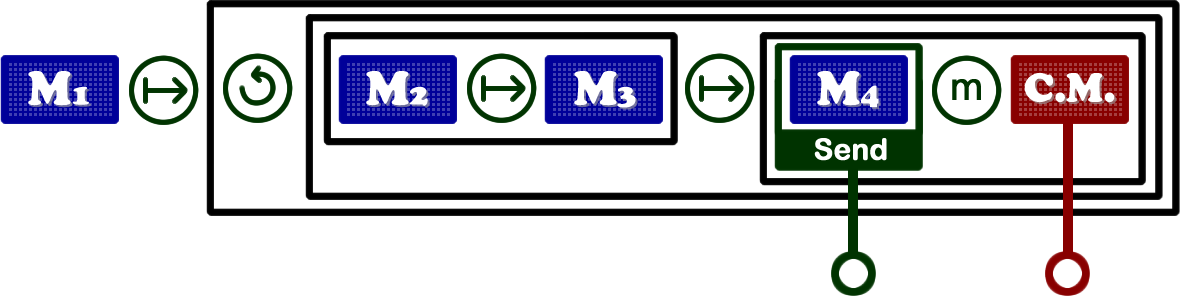
\includegraphics[width=0.9\columnwidth]{as_1}
	}\\
	\subfloat[][Definition de la strategie de communication]{
		\label{subfig:comm}
		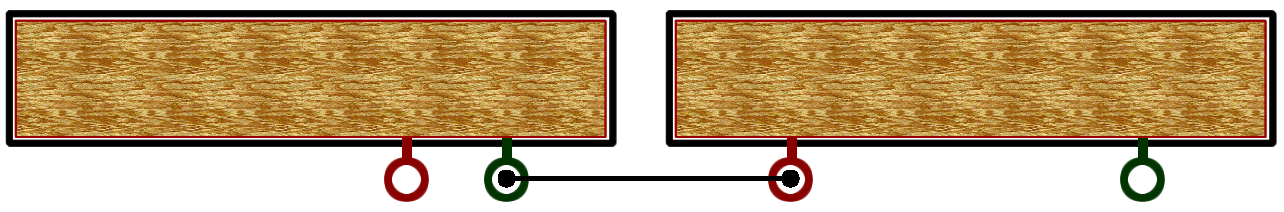
\includegraphics[width=0.9\columnwidth]{conn_1}
	}
	\caption[]{Construire des solveurs parallèles avec \posl{}}
	\label{fig:posl}
\end{figure}%fr

Les sous-sections suivantes expliquent en détail chacune des étapes ci-dessus.

\subsection{Computation module}

Un \om{}  est la plus basique  et abstraite manière de  définir un composant de calcul. Il reçoit une entrée, exécute un algorithme interne et retourne une sortie. Dans ce papier, nous utilisons ce concept afin de décrire et  définir les composants de base d'un  solveur, qui seront assemblés par l'\as.  

Un \om{} représente un  morceau de l'algorithme  du solveur  qui est susceptible de changer au cours de  l'exécution.   Il  peut  être
dynamiquement remplacé  ou combiné avec d'autres  \oms, puisque les \oms{}  sont  également  des   informations  échangeables  entre  les
solveurs. De  cette manière,  le  solveur  peut changer/adapter  son comportement à  chaud, en combinant  ses \oms{} avec ceux  des autres solveurs. Ils sont  représentés par  des blocs  bleus dans  la figure~\ref{fig:posl}.

\begin{definition}\label{def:module} \textbf{(Computation Module)}
Un \om{} $\mathcal{O}m$ est une application définie par :
\begin{equation}
 \mathcal{C}m:\mathcal{I} \rightarrow \mathcal{O}
\end{equation}
\end{definition}

Dans (\ref{def:module}),  la nature de $\mathcal{D}$  et $\mathcal{I}$ dépend du type de \om{}.  Ils peuvent être soit une configuration, ou  un  ensemble de  configurations, ou un ensemble de  valeurs  de différents types de données, etc.

Soit une méta-heuristique de recherche locale, basée sur un algorithme bien connu, comme par exemple {\it Tabu Search}. Prenons l'exemple d'un  \om{} retournant  le voisinage  d'une configuration  donnée, pour une certaine métrique de voisinage. Cet \om{} peut être défini par la fonction suivante:

\begin{equation}
\mathcal{C}m:D_1\times D_2\times\dots\times D_n \rightarrow 2^{D_1\times D_2\times\dots\times D_n}
\end{equation}

où $D_i$  représente  la  définition  des  domaines  de  chacune  des variables de la configuration d'entrée.

\subsection{Communication module}

Les \opchs{} sont  les composants des solveurs en charge  de la réception des informations  communiquées entre  solveurs. Ils  peuvent interagir
avec les  \oms, en fonction de l'\as. Les \opchs{} jouent  le rôle de prise, permettant aux  solveurs de  se  brancher et  de recevoir  des informations. Il sont représentés en rouge dans la figure~\ref{subfig:modules}.

Un \opch{} peut recevoir deux types d'informations, provenant toujours d'un solveur tiers : des données et des \oms. En  ce qui concerne les \oms, leur  communication peut  se faire  via la  transmission d'identifiants permettant à chaque solveur de les instancier.

Pour faire  la distinction entre  les deux différents types  de \opchs, nous appelons \INTROdopch{} les \opchs{} responsables de la réception de données  et \INTROoopch{} ceux s'occupant de la réception et de l'instanciation de \oms.

\defname{Data communication module}{
Un \dopch{} $\mathcal{C}h$ est un composant produisant une application définie comme suit : 
\begin{equation}
\label{def:dopench}
\mathcal{C}h: I\times\left\{D\cup\left\{NULL\right\}\right\} \rightarrow D \cup \left\{NULL\right\}
\end{equation}
et retournant l'information  $\mathcal{I}$ provenant d'un solveur tiers,quelque soit l'entrée $\mathcal{U}$.
}

\begin{definition}\label{def:oopench} \textbf{(Object communication module)} 
Si nous notons $\mathbf{M}$ l'espace  de  tous  les \oms{} de la définition~\ref{def:module}, alors un \oopch{} $\mathcal{C}h$ est  un composant produisant un \om{}  venant d'un solveur tiers défini ainsi :
\begin{equation}
\mathcal{C}h:I\times\left\{\mathbf{M}\cup\left\{NULL\right\}\right\} \rightarrow O\cup\left\{NULL\right\}
\end{equation}
\end{definition}

Puisque les \opchs{}  reçoivent  des  informations  provenant  d'autres solveurs sans pour autant avoir de contrôle sur celles-ci, il est  nécessaire  de  définir   l'information  {\it  NULL},  signifiant l'absence  d'information.  La  figure~\ref{fig:ochperform}  montre  le mécanisme interne d'un  \opch{}. Si un \dopch{} reçoit une  information,  celle-ci   est  automatiquement  retournée  (figure~\ref{subfig:doch},  lignes bleues).  Si un  \oopch{} reçoit un \om{}, ce dernier est instancié et exécuté avec l'entrée de l'\opch, et  le résultat  est retourné  (figure \ref{subfig:ooch}, lignes bleues). Dans les deux  cas, si aucune information n'est reçue, l'\opch{}  retourne l'objet  {\it NULL}  (figure \ref{fig:ochperform}, lignes rouges).

\begin{figure}
	\centering
	\subfloat[][Data \opch]{
		\label{subfig:doch}
		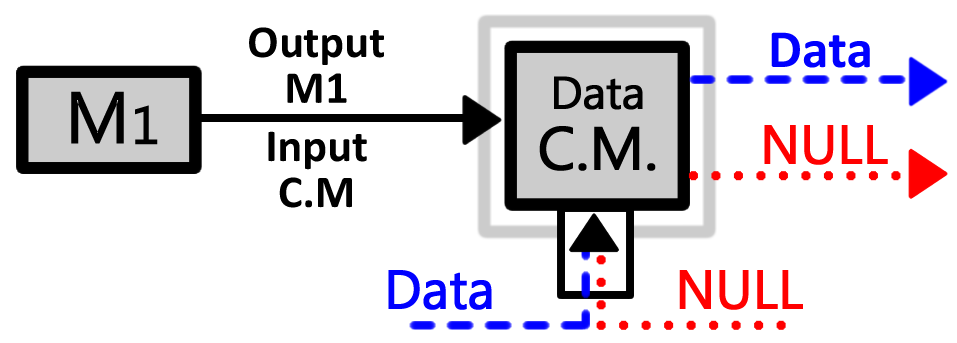
\includegraphics[width=0.7\linewidth]{D_OCh} %[width=0.2\textwidth]{muta1}
	}
	\\%\hspace{0.05\textwidth}%
	\subfloat[][Object \opch]{%
		\label{subfig:ooch}
		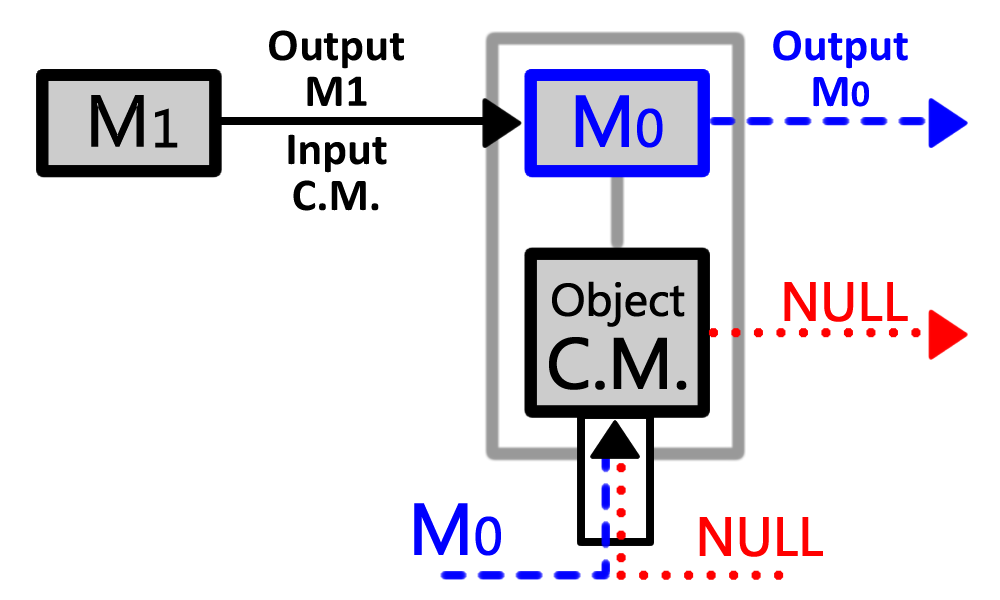
\includegraphics[width=0.7\linewidth]{O_OCh}%[width=0.2\textwidth]{muta2}
	}
	\caption[]{Mécanisme interne du \opch}
	\label{fig:ochperform}
\end{figure}%fr

\subsection{Abstract solver}

L'\as{}  est le c\oe{}ur du solveur. Il joint les \oms{} et les \opchs{} de  manière cohérente, tout en leur restant  indépendant. Ceci signifie  qu'elle peut  changer ou  être modifiée  durant l'exécution, sans altérer  l'algorithme général  et en  respectant la  structure du solveur.  À  travers  l'\as, on peut décider également des informations à envoyer aux autres solveurs. \new{Chaque fois que nous combinons certains composants en utilisant des opérateurs \posl{}, nous créons un \INTROm.}

\begin{definition}
\label{def:cm}
Noté par la lettre $\mathcal{M}$, un {\bf \m} est:
\begin{enumerate}\renewcommand{\labelitemi}{\scriptsize$\blacksquare$}
\item un \om{}; ou
\item un \opch{}; ou
\item $\left[\mbox{OP } \mathcal{M}\right]$, \new{la composition d'un module $\mathcal{M}$ exécuté sequentielement, en retournant une sortie, en dépendant de la nature de l'opérateur unaire \emph{OP};} ou \label{subdef:seq_uni}
\item $\left[\mathcal{M}_1 \mbox{ OP } \mathcal{M}_2\right]$, \new{la composition de deux modules $\mathcal{M}_1$ et $\mathcal{M}_2$ exécuté séquentiellement, en retournant une sortie, en dépendant de la nature de l'opérateur binaire \emph{OP}.}\label{subdef:seq}
\item $\left[\mathcal{M}_1 \mbox{ OP } \mathcal{M}_2\right]$, \new{la composition de deux modules $\mathcal{M}_1$ et $\mathcal{M}_2$ exécuté, en retournant une sortie, en dépendant de la nature de l'opérateur binaire \emph{OP}. Ces deux opérateurs vont être exécutes en parallèle si et seulement si \emph{OP} support le parallélisme, ou il lance une exception en cas contraire.}\label{subdef:par}
\end{enumerate}
Nous notons par $\mathbf{M}$ l'espace des \ms, et nous appelons \cms{} à la composition de \ms{} présentés en \ref{subdef:seq_uni} \ref{subdef:seq}, et/ou \ref{subdef:par}.
\end{definition}

Pour illustrer la définition~\ref{def:cm}, la figure~\ref{fig:cm} montre graphiquement le concept de \cm.
\begin{figure}
	\centering
	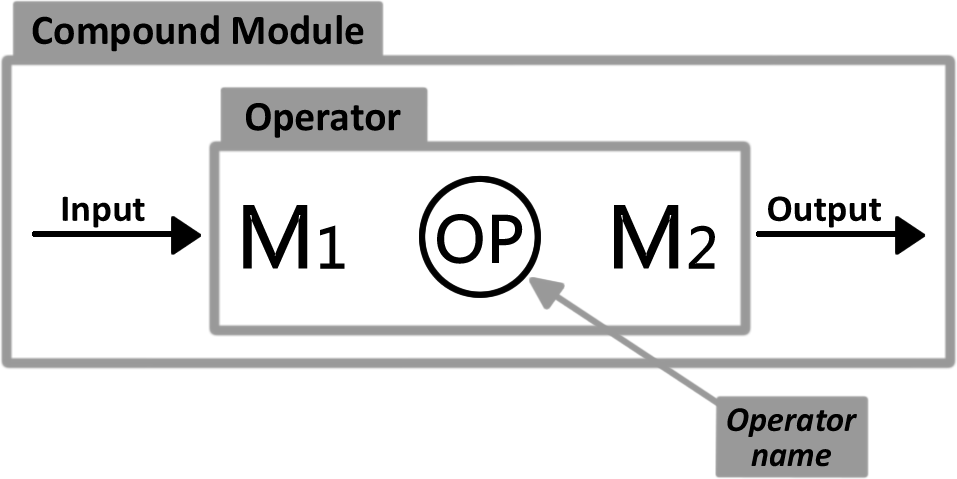
\includegraphics[width=0.7\linewidth]{cm} %[width=0.2\textwidth]{muta1}
	\caption[]{Un \cm}
	\label{fig:cm}
\end{figure}%fr

Dans le  cas particulier  où un  des \cms{}  impliqués est  un \opch{}, chaque opérateur gère l'information {\it NULL} à sa manière.

Afin   de  grouper   des   modules,  nous   utiliserons  la   notation $\left|.\right|$ comme un groupe générique qui pourra être indifféremment interprété comme $[.]$ ou comme $\lbk . \rbk_p$.

L'opérateur suivant nous permet d'exécuter deux modules séquentiellement, l'un après l'autre.

\begin{definition}\label{def:seqexec} {\bf (Sequential Execution Operator)} 
Soient
\begin{inparaenum}[i)]
	\item $\mathcal{M}_1 : \mathcal{D}_1 \rightarrow \mathcal{I}_1$ et
	\item $\mathcal{M}_2 : \mathcal{D}_2 \rightarrow \mathcal{I}_2$.
\end{inparaenum}
deux \ms{} différents. \new{Alors l'opération  $\left|\mathcal{M}_1\poslop{\mapsto}\mathcal{M}_2\right|$ définit le \cm{} $\mathcal{M}_{seq}$ comme le résultat de l'exécution de $\mathcal{M}_1$ suivi de $\mathcal{M}_2$.}

\[
\mathcal{M}_{seq}:\mathcal{D}_1 \rightarrow \mathcal{I}_2
\]
\end{definition}


L'opérateur  présenté  dans  la  définition~\ref{def:seqexec}  est  un exemple d'opérateur ne  supportant pas une exécution  parallèle de ses \cms impliqués, puisque l'entrée du second \cm{} est la sortie du premier.

%\begin{tabular}{ll}
%	$\left[\mathcal{M}_1\poslop{\mapsto}\mathcal{M}_2\right]$ & \textcolor{darkgreen}{\bf OK!}\\
%	$\lbk\mathcal{M}_1\poslop{\mapsto}\mathcal{M}_2\rbk_p$ & \textcolor{red}{\bf Impossible}
%\end{tabular}

L'opérateur suivant  est utile  pour exécuter des  modules séquentiels créant des branchements de calcul selon une condition booléenne :

\begin{definition}\label{op:conditional}
{\bf (Conditional Execution Operator)} Soient 
\begin{inparaenum}[i)]
	\item $\mathcal{M}_1 : \mathcal{D} \rightarrow \mathcal{I}_1$ et 
	\item $\mathcal{M}_2 : \mathcal{D} \rightarrow \mathcal{I}_2$,
\end{inparaenum} 
deux \ms{} différents. \new{Alors l'opération $\left|\mathcal{M}_1\circled{?}_{<cond>}\mathcal{M}_2\right|$ définit le \cm{} $\mathcal{M}_{cond}$ le résultat de l'exécution en séquentiel de $\mathcal{M}_1$ si $<cond>$ es {\bf vrai} or $\mathcal{M}_2$, autrement}:

\[
\mathcal{M}_{cond}:\mathcal{D} \rightarrow \mathcal{I}_1 \cup \mathcal{I}_2 
\]
\end{definition}

Nous pouvons exécuter séquentiellement  des modules créant des boucles de calcul, en définissant les \cms{} avec un autre opérateur conditionnel:

\begin{definition}\label{op:cyclic}
{\bf (Cyclic Execution Operator)} Soit $\mathcal{M} : \mathcal{D} \rightarrow \mathcal{I}$ un \m, où $\mathcal{I} \subseteq \mathcal{D}$. \new{Alors, l'opération $\left|\circlearrowleft_{<cond>}\mathcal{M}\right|$ définit le \cm{} $\mathcal{M}_{cyc}$ en répétant séquentiellement l'exécution de $\mathcal{M}$ tant que $<cond>$ est {\bf vrai}:}

\[
\mathcal{M}_{cyc}:\mathcal{D} \rightarrow \mathcal{I} 
\]
\end{definition}

%Dans la figure~\ref{fig:ex1}, on  présente un exemple simple combinant des \ms utilisant les opérateurs de \posl{} introduis ci-dessus. L'algorithme~\ref{algo:ex1} montre le code correspondant. Cet exemple montre  trois \ms{} faisant  partie d'un \cm{} avec pour but de générer  une configuration initiale à partir de laquelle débutera un solveur de recherche locale. Nous avons ainsi :
%
%\begin{itemize}
%\item $\mathcal{M}_1$, générant une configuration aléatoire.
%\item {$\mathcal{M}_2$, sélectionnant une variable aléatoire  d'une  configuration donnée, et recopiant sa valeur dans une autre variable.}
%\item $\mathcal{M}_3$, stockant la meilleure configuration trouvée.
%\end{itemize}

%{Dans cet exemple, l'\module{} $\mathcal{M}_2$ est d'abord exécuté, suivi
%de $\mathcal{M}_3$  si tous les  éléments de la  configuration générée
%sont  différents} (\verb!<  cond  >!). {Sinon,  seul l'\module{}
%$\mathcal{M}_3$ est  exécuté. Cette  opération est répétée  un certain
%nombre de fois} (\verb!< stop_cond >!).
%
%\figalgosbs{
%	\centering
%% eric
%%	\includegraphics[width=\linewidth]{Ex1v2.eps}
%	\includegraphics[width=0.8\linewidth]{Ex1v2}
%	\caption{}\label{fig:ex1}
%}{
%%\caption{\af{} code for Figure \ref{fig:ex1}}
%\caption{Code \af{} de la figure \ref{fig:ex1}}
%\dontprintsemicolon
%\SetNoline
%
%\While{$<\text{stop\_cond}>$}{		
%	$\left[\mathcal{M}_1 \xmapsto[<cond>]{} \left\{\mathcal{M}_2;\left[\mathcal{M}_2 \longmapsto\mathcal{M}_3\right]\right\}\right]$\;			
%}
%\label{algo:ex1}
%}%fr

\posl{} offre la possibilité de faire muter les solveurs. En fonction de l'opération, un  ou plusieurs \m{} opérande(s) sera exécutée(s), mais seule la sortie de l'un d'entre  eux sera retournée par le \cm. Nous présentons  ces opérateurs  dans deux  définitions, groupant  ceux qui exécutent uniquement un opérande  de \m{}~(définition~\ref{op:rho} et \ref{op:or}) et ceux exécutant les deux opérandes~(définition~\ref{op:min}, \ref{op:max} et~\ref{op:race}).

\begin{definition}\label{op:rho}
{\bf Random Choice Operator} Soient
\begin{inparaenum}[i)]
	\item $\mathcal{M}_1 : \mathcal{D} \rightarrow \mathcal{I}_1$ et
	\item $\mathcal{M}_2 : \mathcal{D} \rightarrow \mathcal{I}_2$,
\end{inparaenum} 
deux \ms{} différents, et un numéro réel $\rho \in (0,1)$. \new{Alors, l'operation $\left|M_1\circled{$\rho$}\mathcal{M}_2\right|$ définit le \cm{} $\mathcal{M}_{rho}$ qui exécute $\mathcal{M}_1$ en suivant une probabilité $\rho$, ou en exécutant $\mathcal{M}_2$ en suivant une probabilité $(1-\rho)$:}

\[
\mathcal{M}_{rho}:\mathcal{D} \rightarrow \mathcal{I}_1 \cup \mathcal{I}_2 
\]
\end{definition}

\begin{definition}\label{op:or}
{\bf Not {\it NULL} Execution Operator} Soient
\begin{inparaenum}[i)]
	\item $\mathcal{M}_1 : \mathcal{D} \rightarrow \mathcal{I}_1$ et  
	\item $\mathcal{M}_2 : \mathcal{D} \rightarrow \mathcal{I}_2$,
\end{inparaenum} 
deux \ms{} différents. \new{Alors, l'operation $\left|\mathcal{M}_1\circled{$\vee$}\mathcal{M}_2\right|$ définit le \cm{} $\mathcal{M}_{non}$ qui exécute $\mathcal{M}_1$ et retourne une sortie si elle n'est pas{\it NULL}, ou exécute $\mathcal{M}_2$ et retourne une sortie autrement:}

\[
\mathcal{M}_{non}:\mathcal{D} \rightarrow \mathcal{I}_1 \cup \mathcal{I}_2 
\]
\end{definition}

La définition suivante  fait appelle aux notions  de {\it parallélisme coopératif} et de {\it parallélisme compétitif}. Nous disons qu'il y a  parallélisme  coopératif  quand  deux  unités  de  calcul  ou  plus s'exécutent simultanément, et que le résultat obtenu provient de la combinaison des  résultats calculés par  chaque unité de  calcul (voir définitions~\ref{op:min} et \ref{op:max}). À l'opposé, nous  considérons qu'il y  a parallélisme compétitif  lorsque le résultat obtenu  est une solution ne provenant  que d'un seul processus exécuté  en parallèle; en  général   le  premier   processus  à  terminer   (voir  définition \ref{op:race}). 

\begin{definition}\label{op:min}
{\bf Minimum Operator } Soient 
\begin{enumerate}%\begin{inparaenum}[i)]
	\item $\mathcal{M}_1 : \mathcal{D} \rightarrow \mathcal{I}_1$ et
	\item $\mathcal{M}_2 : \mathcal{D} \rightarrow \mathcal{I}_2$,
\end{enumerate}%\end{inparaenum} 
deux \ms{} différents. \new{Soient aussi $o_1$ et $o_2$ les sorties de $\mathcal{M}_1$ et $\mathcal{M}_2$, respectivement. Nous assumons qu'il existe un ordre total dans $I_1 \cup I_2$ où l'objet \emph{NULL} est la plus grand valeur. Alors, l'opération $\left|\mathcal{M}_1\circled{m}\mathcal{M}_2\right|$ définit le \cm{} $\mathcal{M}_{min}$ qui exécute $\mathcal{M}_1$ et $\mathcal{M}_2$, et retourne $\min\left\{o_1,o_2\right\}$:}

\[
\mathcal{M}_{min}:\mathcal{D} \rightarrow \mathcal{I}_1 \cup \mathcal{I}_2 
\]
\end{definition}

De la même manière nous définissons l'opérateur \textbf{Maximum}:

\begin{definition}\label{op:max}
{\bf Minimum Operator} Soient 
\begin{enumerate}%\begin{inparaenum}[i)]
	\item $\mathcal{M}_1 : \mathcal{D} \rightarrow \mathcal{I}_1$ et
	\item $\mathcal{M}_2 : \mathcal{D} \rightarrow \mathcal{I}_2$,
\end{enumerate}%\end{inparaenum} 
deux \ms{} différents. \new{Soient aussi $o_1$ et $o_2$ les sorties de $\mathcal{M}_1$ et $\mathcal{M}_2$, respectivement. Nous assumons qu'il existe un ordre total dans $I_1 \cup I_2$ où l'objet \emph{NULL} est la plus petite valeur. Alors, l'opération $\left|\mathcal{M}_1\circled{M}\mathcal{M}_2\right|$ définit le \cm{} $\mathcal{M}_{max}$ qui exécute $\mathcal{M}_1$ et $\mathcal{M}_2$, et retourne $\max\left\{o_1,o_2\right\}$:}

\[
\mathcal{M}_{max}:\mathcal{D} \rightarrow \mathcal{I}_1 \cup \mathcal{I}_2 
\]
\end{definition}

%\poslexample{The {\bf minimum operator} can be applied in the previews example to obtain an interesting behavior: When applying the acceptance criteria, suppose that we want to receive a configuration from another solver, to compare it with ours and select the one with the lowest cost. We can do that by applying the $\circled{m}$ operator to combine the \om{} $A$ with a \opch{} $C.M.$ (see Figure\ref{fig:min_example}):
%$$\left[I\poslop{\mapsto}\left[\circlearrowleft\left[\left[V\poslop{\mapsto}S\right]\poslop{\mapsto}\lbk A\poslop{m}C.M.\rbk_p\right]\right]\right]$$
%Notice that in this example, I can use the grouper $\lbk .\rbk_p$ since the {\bf minimum operator} supports parallelism.}
%
%\begin{figure}[h]
%	\centering	
%	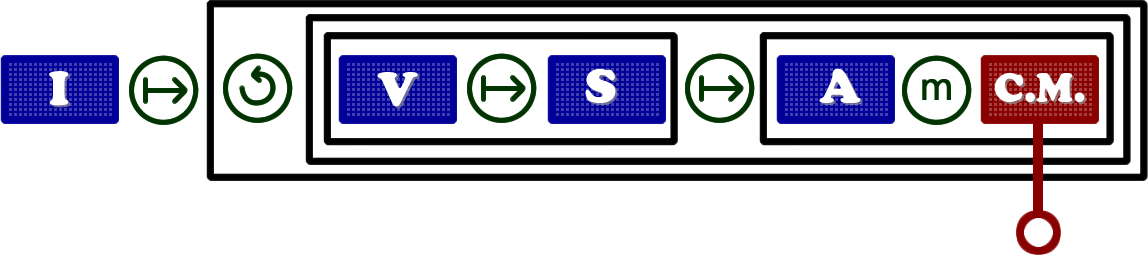
\includegraphics[width=0.6\linewidth]{min.png}
%	\caption{Using {\bf minimum} operator}\label{fig:min_example}
%\end{figure}

\begin{definition}\label{op:race}
{\bf Race Operator} Soient
\begin{inparaenum}[i)]
	\item $\mathcal{M}_1 : \mathcal{D} \rightarrow \mathcal{I}_1$  et
	\item $\mathcal{M}_2 : \mathcal{D} \rightarrow \mathcal{I}_2$,
\end{inparaenum} deux \ms{} différents, où $\mathcal{D}_1 \subseteq \mathcal{D}_2$ et $\mathcal{I}_1 \subset \mathcal{I}_2$. \new{Alors, l'opération $\left|\mathcal{M}_1\circled{$\shortdownarrow$}\mathcal{M}_2\right|$ définit le \cm{} $\mathcal{M}_{race}$ qui exécute les deux \ms{} $\mathcal{M}_1$ et $\mathcal{M}_2$, et retourne la sortie du \m{} qui termine en premier:}

\[
\mathcal{M}_{race}:\mathcal{D} \rightarrow \mathcal{I}_1 \cup \mathcal{I}_2 
\]
\end{definition}

%\figalgosbs{\
%	\centering
%% eric
%%	\includegraphics[width=\linewidth]{Ex2v2.eps}
%	\includegraphics[width=0.8\linewidth]{Ex2v2}
%	\caption{}\label{fig:ex2}
%}{
%%\caption{\af{} code for Figure \ref{fig:ex2}}
%\caption{Code \af{} de la figure \ref{fig:ex2}}
%\dontprintsemicolon
%\SetNoline	
%$\mathcal{M}_1 \longmapsto \lbk\mathcal{M}_2\circled{$\times$}\lbk\mathcal{M}_3 \circled{$\shortdownarrow$} \mathcal{M}_4\rbk_p\rbk_p\longmapsto\mathcal{M}_5$\;			
%\label{algo:ex2}
%}%fr
%
%Nous  illustrons un  de  ces  trois opérateurs  dans  l'exemple de  la
%figure~\ref{fig:ex2}. Les modules rentrant en jeu sont :
%
%\begin{itemize}
%	\item $\mathcal{M}_1$, retournant une configuration
%	\item $\mathcal{M}_2$, calculant un paramètre de tolérance $\epsilon$
%	\item   $\mathcal{M}_3$  et   $\mathcal{M}_4$,  calculant   le
%          voisinage  $\mathcal{N}$ de  la  configuration provenant  de
%          $\mathcal{M}_1$.  Ces deux  \modules    calcule  $\mathcal{N}$ de  manière
%          différente, mais ils sont combinés de façon à ce que seul la
%          sortie du premier module terminant son calcul soit retournée.
%	\item  $\mathcal{M}_5$, sélectionnant  une configuration  dans
%          $\mathcal{N}$ améliorant  le coût  global avec  un tolérance
%          $\epsilon$,  à  la  manière   du  {\it  Threshold  Accepting
%            Method}~\cite{Boussaid2013}
%\end{itemize}
%
%Dans   l'algorithme~\ref{algo:ex2},   les    \ms   $\mathcal{M}_3$   et
%$\mathcal{M}_4$ sont  exécutés en  parallèle, mais  seule la  sortie du
%premier module à terminer son calcul sera retournée. 
%
%De  la   même  manière,  le   \cm{}  composé  de   $\mathcal{M}_3$  et
%$\mathcal{M}_4$ peut  être exécuté en parallèle  avec $\mathcal{M}_2$,
%parce qu'ils sont  indépendants l'un de l'autre et  que l'opérateur le
%permet. Il est important de souligner qu'ils peuvent être exécutés par
%l'opérateur $\circled{$\times$}$, puisqu'ils reçoivent la même entrée.

Les  opérateurs   introduits  par  les   définitions~\ref{op:rho}, \ref{op:or} et \ref{op:min} sont très  utiles en  terme de  partage d'informations entre   solveurs, mais également en terme de partage de comportements. Si un  des opérandes est un  \opch{} alors l'opérateur peut recevoir le \om{} d'un autre solveur, donnant la possibilité d'instancier ce module dans le solveur le réceptionnant. L'opérateur va soit instancier le module s'il  n'est pas {\it NULL} et l'exécuter, soit exécuter le module donné par le second opérande.

Maintenant, nous définissons les  opérateurs nous permettant d'envoyer de  l'information vers  d'autres  solveurs. Deux  types d'envois  sont possibles :
\begin{inparaenum}[i)]
	\item on exécute un \m{} et on envoie sa sortie,
	\item ou on envoie le \m{} lui-même.
\end{inparaenum}

\begin{definition}\label{op:osend}
{\bf Sending Data Operator} Soit $\mathcal{M} : \mathcal{D} \rightarrow \mathcal{I}$ un \m. \new{Alors, l'opération $\left|\senddataop{\mathcal{M}}\right|$ définit le \cm{} $\mathcal{M}_{sendD}$ qui exécute le \m{} $\mathcal{M}$ puis envoie la sortie vers un \opch:}

\[
\mathcal{M}_{sendD}:\mathcal{D} \rightarrow \mathcal{I}
\]
\end{definition}

\begin{definition}\label{op:msend}
{\bf Sending Module Operator} Soit $\mathcal{M} : \mathcal{D} \rightarrow \mathcal{I}$ un \m. \new{Alors, l'opération $\left|\sendmoduleop{\mathcal{M}}\right|$ définit le \cm{} $\mathcal{M}_{sendM}$ qui exécute le \m{} $\mathcal{M}$, puis envoie le \m{} lui même  vers un \opch:}

\[
\mathcal{M}_{sendM}:\mathcal{D} \rightarrow \mathcal{I}
\]
\end{definition}

Avec  les opérateurs  présentés jusqu'ici,  nous sommes  en mesure  de concevoir les \ass{} (ou algorithme) de résolution d'un problème de contraintes. Une fois un  tel \as{} définie, on  peut changer les composants (\oms{} et \opchs) auxquels elle fait appel, permettant  ainsi d'implémenter différents solveurs à partir du même \as{} mais composés de différents \ms, du moment que ces derniers respectent  la signature attendue, à savoir le types des entrées et sorties.

\new{Un \as{} est déclaré comme suit: après déclarer les noms de l'\mbox{\tet{\bf \as}} ({\it name}), la première ligne définit la liste des \oms{} abstraites ($\mathcal{L}^m$), la seconde ligne, la liste des \opchs{} abstraites ($\mathbf{M}$), puis l'algorithme du solver est définit comment le corps su solver (the root \cm{} $\mathbf{M}$), entre \mbox{\tet{\bf begin}} et \mbox{\tet{\bf end}}.}

\new{Un \as{} peut être déclaré par l'expression régulière suivante:}

\begin{center}
\tet{\bf abstract solver} {\it name} \tet{\bf computation}: $\mathcal{L}^m$ (\tet{\bf communication}: $\mathcal{L}^c$)? \tet{\bf begin} $\mathbf{M}$ \tet{\bf end}
\end{center}

Par exemple, l'algorithme~\ref{algo:as_example} montre l'\as{} correspondant a la figure~\ref{subfig:as}.

\begin{algorithm}[h]
\dontprintsemicolon
\SetNoline
\SetKwProg{myproc}{}{}{}
\myproc{\tet{\bf abstract solver} as\_01\;
\tet{\bf computation} : $I, V, S, A$ \; 
\tet{\bf connection}: $C.M.$}{
	\Begin{
		$I \poslop{\mapsto}$\\
		\While{$\left(\textbf{\Iter < } K_1\right)$}{
			$\left[V\poslop{\mapsto}S\poslop{\mapsto}\left[C.M.\poslop{m} \senddataop{A}\right]\right]$%
		}
	}
}
\caption{Pseudo-code \posl{} pour l'\as{} de la figure~\ref{subfig:as}}\label{algo:as_example}
\end{algorithm}

\subsection{Créer les solveurs}

\new{Maintenant on peut créer les solveurs en instanciant les \ms. Il est possible de faire ceci en spécifiant que un \mbox{\tet{\bf solver}} donné doit implémenter (en utilisant le mot clé \mbox{\tet{\bf implements}}) un \as{} donné, suivi par la liste de \omprefix{} puis \opchs{}. Ces \ms{} doivent correspondre avec les signatures exigé par l'\as.}

\begin{algorithm}[h]
\dontprintsemicolon
\SetNoline
\SetKwProg{myproc}{}{}{}
\tet{\bf solver} solver\_01 \tet{\bf implements} as\_01\;
\tet{\bf computation} : $I_{rand}, V_{1ch}, S_{best}, A_{AI}$ \; 
\tet{\bf connection}: $CM_{last}$\;
\caption{Une instanciation de l'\as{} présenté dans l'algorithme~\ref{algo:as_example}}\label{algo:solver_def}
\end{algorithm}

\subsection{Connecter les solveurs : créer le \soset}

\new{La dernière étape est connecter les solveurs entre eux. \posl{} fournit des outils pour créer des stratégies de communication très facilement. L'ensemble des solveurs connectés qui seront exécutés en parallèle pour résoudre un CSP s'appelle \INTROsoset{}.}

Les communications sont établies en respectant les règles suivantes :
\begin{enumerate}
\item  À chaque  fois qu'un  solveur  envoie une  information via  les opérateurs  $\llparenthesis .\rrparenthesis^{d}$  ou $\llparenthesis   .\rrparenthesis^{m}$, il créé une {\it prise mâle de communication} 
\item À  chaque fois qu'un  solveur contient  un \opch{}, il  créé une {\it prise femelle de communication} 
\item Les solveurs peuvent être connectés entre eux en reliant {\it prises mâles} et {\it femelles}.
\end{enumerate}

Avec l'opérateur~$(\cdot)$, nous  pouvons  avoir  accès aux  \oms{} envoyant une information et aux noms des \opchs d'un solveur. Par exemple : $Solver_1\cdot\mathcal{M}_1$ fournit  un accès à le \om{} $\mathcal{M}_1$ du $Solver_1$ si et seulement s'il est utilisé par l'opérateur  $\llparenthesis .\rrparenthesis^{o}$  (ou $\llparenthesis.\rrparenthesis^{m}$), et $Solver_2\cdot\mathcal{C}h_2$ fournit un accès au \opch{} $\mathcal{C}h_2$ de $Solver_2$.

Maintenant, nous définissons les opérateurs de communication que \posl{} fournit.

\begin{definition}\label{op_conn:1to1}
{\bf Connection One-to-One Operator} Soient
\begin{enumerate}
\item $\mathcal{J} = \left[\mathcal{S}_0\cdot \mathcal{M}_0, \mathcal{S}_1\cdot \mathcal{M}_1,\dots, \mathcal{S}_{N-1}\cdot \mathcal{M}_{N-1}\right]$ une liste de  {\it prises mâles}, et
\item $\mathcal{O} = \left[\mathcal{Z}_0\cdot \mathcal{CM}_0, \mathcal{Z}_1\cdot \mathcal{CM}_1,\dots, \mathcal{Z}_{N-1}\cdot \mathcal{CM}_{N-1}\right]$ une liste de {\it prises femelles}
\end{enumerate} Alors, l'opération
\[
\mathcal{J} \poslop{\rightarrow} \mathcal{O}
\]
\new{connecte chaque {\it prise mâles} $\mathcal{S}_i\cdot \mathcal{M}_i \in \mathcal{J}$ avec la correspondante {\it prise femelle} $\mathcal{Z}_i\cdot \mathcal{CM}_i \in \mathcal{O}$, $\forall\textbf{ }0 \leq i \leq N-1$ (voir figure~\ref{subfig:comm_simple}).}
\end{definition}

\begin{definition}\label{op_conn:1ton}
{\bf Connection One-to-N Operator} Soient 
\begin{enumerate} 
\item $\mathcal{J} = \left[\mathcal{S}_0\cdot \mathcal{M}_0, \mathcal{S}_1\cdot \mathcal{M}_1,\dots, \mathcal{S}_{N-1}\cdot \mathcal{M}_{N-1}\right]$ une liste de  {\it prises mâles}, et
\item $\mathcal{O} = \left[\mathcal{Z}_0\cdot \mathcal{CM}_0, \mathcal{Z}_1\cdot \mathcal{CM}_1,\dots, \mathcal{Z}_{M-1}\cdot \mathcal{CM}_{M-1}\right]$ une liste de {\it prises femelles}
\end{enumerate} Alors, l'opération
\[
\mathcal{J} \poslop{\rightsquigarrow} \mathcal{O}
\]
\new{connecte chaque {\it prise mâles} $\mathcal{S}_i\cdot \mathcal{M}_i \in \mathcal{J}$ avec chaque {\it prise femelle} $\mathcal{Z}_j\cdot \mathcal{CM}_j \in \mathcal{O}$, $\forall\textbf{ }0 \leq i \leq N-1$ et $0 \leq j \leq M-1$ (see Figure~\ref{subfig:comm_diff}).}
\end{definition}


\posl{} permet aussi de déclarer des solveurs non communicatifs pour les exécuter en parallèle, en déclarant seulement la liste des noms:
\[
\left[\mathcal{S}_0, \mathcal{S}_1, \dots, \mathcal{S}_{N-1}\right]
\]

\begin{figure}[h]
\centering
\subfloat[][Communication 1 à 1]{
	\label{subfig:comm_simple}
	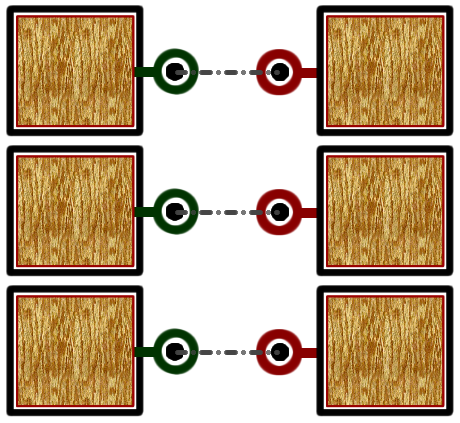
\includegraphics[width=0.4\columnwidth]{comm_11.png}
}
\hspace{0.05\textwidth}%
\subfloat[][Communication 1 à N]{%
	\label{subfig:comm_diff}
	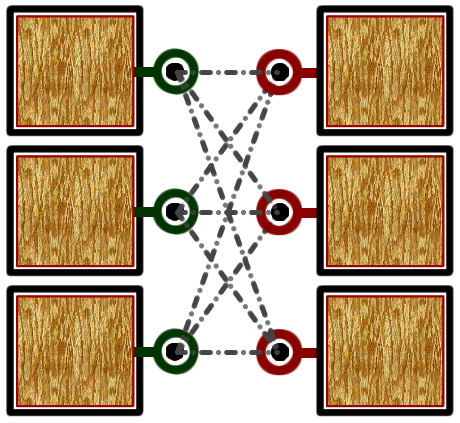
\includegraphics[width=0.4\columnwidth]{comm_1n.png}
}
\caption[]{Représentation graphique des opérateurs de communication}
\label{fig:comm}
\end{figure}

\posl{} permet de construire des solveurs suivant différentes étapes : 
\begin{enumerate}
\item  L'algorithme du solveur considéré est  exprimé via une décomposition  en modules de calcul. Ces modules sont implémentés à la   manière de {\it fonctions} séparées. Nous appelons \INTROom{} ces morceaux de calcul (figure \ref{subfig:modules}, \new{blocs bleus}). \new{En suite, il faut décider  quelles  sont les  types d'informations que l'on souhaite  recevoir des autres solveurs.  Ces informations sont encapsulées  dans des composants appelés  \opch{},  permettant  de transmettre  des  données entre solveurs (figure \ref{subfig:modules}, \new{bloc rouge})} \label{stages:module}

\item  Une {\it stratégie générique}  est codée  à travers  \posl{}, en utilisant les  opérateurs fournis par le langage appliqués  sur des \new{\ms{} \textit{abstraite} qui représentent les \textit{signatures} des} composants donnés lors l'étape \ref{stages:module}, pour créer \ass. Cette  stratégie   définie  non  seulement  les informations   échangées,  mais   détermine  également   l'exécution parallèle de  composants. Lors  de cette  étape, les  informations à partager sont  transmises via  les opérateurs  ad-hoc. On  peut voir cette étape comme la définition de la colonne vertébrale des solveurs (figure \ref{subfig:as}).

\item  Les solveurs sont créés en instanciant \new{l'\as, par \oms{} et \opch}. %puis en les assemblant 

\item \new{Les solveurs sont assemblés en utilisant les opérateurs de communication fournis par le langage, pour creér des strategies de communication. Cet entité final s'appelle \INTROsoset{} (figure \ref{subfig:comm}).}
\end{enumerate}

\begin{figure}
	\centering
	\subfloat[][Definition du \ms{} et l'\opchs{}]{
		\label{subfig:modules}
		
\includegraphics[width=0.5\columnwidth]{modules_1}
	}\\
	\subfloat[][Definition de l'\as]{%
		\label{subfig:as}
		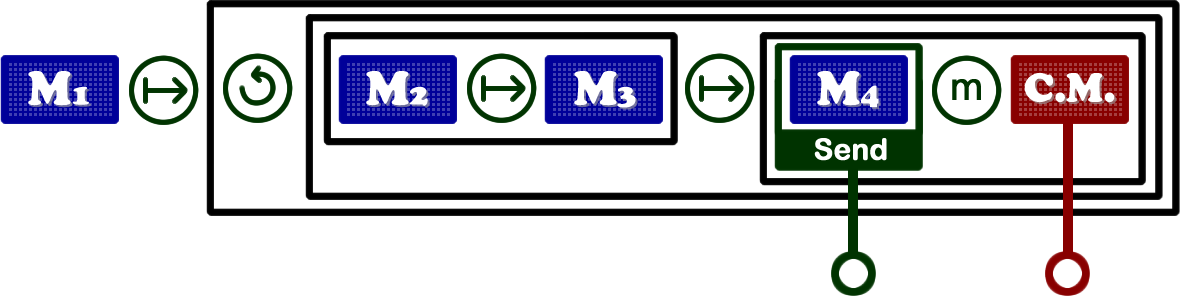
\includegraphics[width=0.9\columnwidth]{as_1}
	}\\
	\subfloat[][Definition de la strategie de communication]{
		\label{subfig:comm}
		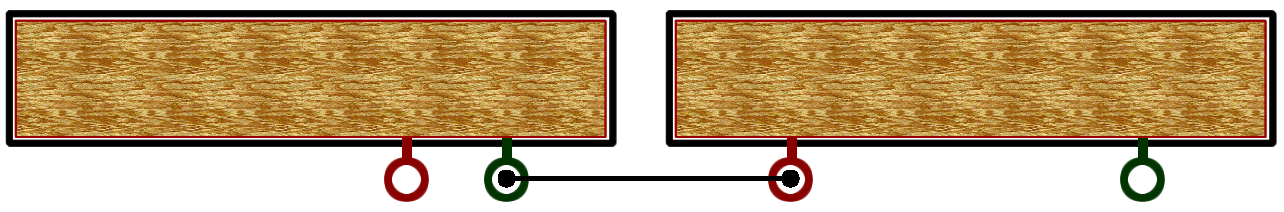
\includegraphics[width=0.9\columnwidth]{conn_1}
	}
	\caption[]{Construire des solveurs parallèles avec \posl{}}
	\label{fig:posl}
\end{figure}%fr

Les sous-sections suivantes expliquent en détail chacune des étapes ci-dessus.

\subsection{Computation module}

Un \om{}  est la plus basique  et abstraite manière de  définir un composant de calcul. Il reçoit une entrée, exécute un algorithme interne et retourne une sortie. Dans ce papier, nous utilisons ce concept afin de décrire et  définir les composants de base d'un  solveur, qui seront assemblés par l'\as.  

Un \om{} représente un  morceau de l'algorithme  du solveur  qui est susceptible de changer au cours de  l'exécution.   Il  peut  être
dynamiquement remplacé  ou combiné avec d'autres  \oms, puisque les \oms{}  sont  également  des   informations  échangeables  entre  les
solveurs. De  cette manière,  le  solveur  peut changer/adapter  son comportement à  chaud, en combinant  ses \oms{} avec ceux  des autres solveurs. Ils sont  représentés par  des blocs  bleus dans  la figure~\ref{fig:posl}.

\begin{definition}\label{def:module} \textbf{(Computation Module)}
Un \om{} $\mathcal{O}m$ est une application définie par :
\begin{equation}
 \mathcal{C}m:\mathcal{I} \rightarrow \mathcal{O}
\end{equation}
\end{definition}

Dans (\ref{def:module}),  la nature de $\mathcal{D}$  et $\mathcal{I}$ dépend du type de \om{}.  Ils peuvent être soit une configuration, ou  un  ensemble de  configurations, ou un ensemble de  valeurs  de différents types de données, etc.

Soit une méta-heuristique de recherche locale, basée sur un algorithme bien connu, comme par exemple {\it Tabu Search}. Prenons l'exemple d'un  \om{} retournant  le voisinage  d'une configuration  donnée, pour une certaine métrique de voisinage. Cet \om{} peut être défini par la fonction suivante:

\begin{equation}
\mathcal{C}m:D_1\times D_2\times\dots\times D_n \rightarrow 2^{D_1\times D_2\times\dots\times D_n}
\end{equation}

où $D_i$  représente  la  définition  des  domaines  de  chacune  des variables de la configuration d'entrée.

\subsection{Communication module}

Les \opchs{} sont  les composants des solveurs en charge  de la réception des informations  communiquées entre  solveurs. Ils  peuvent interagir
avec les  \oms, en fonction de l'\as. Les \opchs{} jouent  le rôle de prise, permettant aux  solveurs de  se  brancher et  de recevoir  des informations. Il sont représentés en rouge dans la figure~\ref{subfig:modules}.

Un \opch{} peut recevoir deux types d'informations, provenant toujours d'un solveur tiers : des données et des \oms. En  ce qui concerne les \oms, leur  communication peut  se faire  via la  transmission d'identifiants permettant à chaque solveur de les instancier.

Pour faire  la distinction entre  les deux différents types  de \opchs, nous appelons \INTROdopch{} les \opchs{} responsables de la réception de données  et \INTROoopch{} ceux s'occupant de la réception et de l'instanciation de \oms.

\defname{Data communication module}{
Un \dopch{} $\mathcal{C}h$ est un composant produisant une application définie comme suit : 
\begin{equation}
\label{def:dopench}
\mathcal{C}h: I\times\left\{D\cup\left\{NULL\right\}\right\} \rightarrow D \cup \left\{NULL\right\}
\end{equation}
et retournant l'information  $\mathcal{I}$ provenant d'un solveur tiers,quelque soit l'entrée $\mathcal{U}$.
}

\begin{definition}\label{def:oopench} \textbf{(Object communication module)} 
Si nous notons $\mathbf{M}$ l'espace  de  tous  les \oms{} de la définition~\ref{def:module}, alors un \oopch{} $\mathcal{C}h$ est  un composant produisant un \om{}  venant d'un solveur tiers défini ainsi :
\begin{equation}
\mathcal{C}h:I\times\left\{\mathbf{M}\cup\left\{NULL\right\}\right\} \rightarrow O\cup\left\{NULL\right\}
\end{equation}
\end{definition}

Puisque les \opchs{}  reçoivent  des  informations  provenant  d'autres solveurs sans pour autant avoir de contrôle sur celles-ci, il est  nécessaire  de  définir   l'information  {\it  NULL},  signifiant l'absence  d'information.  La  figure~\ref{fig:ochperform}  montre  le mécanisme interne d'un  \opch{}. Si un \dopch{} reçoit une  information,  celle-ci   est  automatiquement  retournée  (figure~\ref{subfig:doch},  lignes bleues).  Si un  \oopch{} reçoit un \om{}, ce dernier est instancié et exécuté avec l'entrée de l'\opch, et  le résultat  est retourné  (figure \ref{subfig:ooch}, lignes bleues). Dans les deux  cas, si aucune information n'est reçue, l'\opch{}  retourne l'objet  {\it NULL}  (figure \ref{fig:ochperform}, lignes rouges).

\begin{figure}
	\centering
	\subfloat[][Data \opch]{
		\label{subfig:doch}
		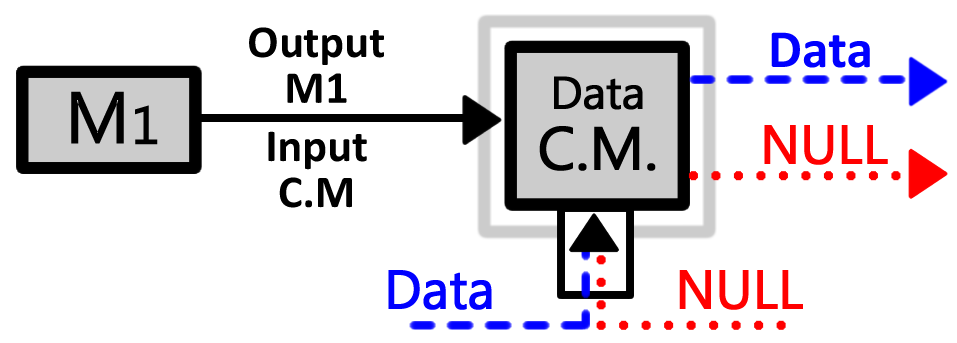
\includegraphics[width=0.7\linewidth]{D_OCh} %[width=0.2\textwidth]{muta1}
	}
	\\%\hspace{0.05\textwidth}%
	\subfloat[][Object \opch]{%
		\label{subfig:ooch}
		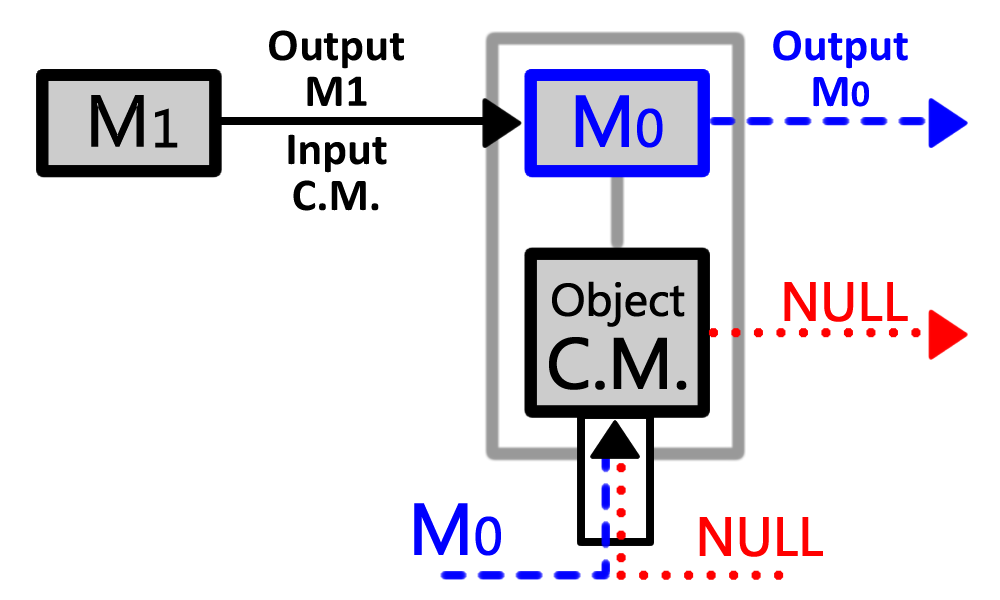
\includegraphics[width=0.7\linewidth]{O_OCh}%[width=0.2\textwidth]{muta2}
	}
	\caption[]{Mécanisme interne du \opch}
	\label{fig:ochperform}
\end{figure}%fr

\subsection{Abstract solver}

L'\as{}  est le c\oe{}ur du solveur. Il joint les \oms{} et les \opchs{} de  manière cohérente, tout en leur restant  indépendant. Ceci signifie  qu'elle peut  changer ou  être modifiée  durant l'exécution, sans altérer  l'algorithme général  et en  respectant la  structure du solveur.  À  travers  l'\as, on peut décider également des informations à envoyer aux autres solveurs. \new{Chaque fois que nous combinons certains composants en utilisant des opérateurs \posl{}, nous créons un \INTROm.}

\begin{definition}
\label{def:cm}
Noté par la lettre $\mathcal{M}$, un {\bf \m} est:
\begin{enumerate}\renewcommand{\labelitemi}{\scriptsize$\blacksquare$}
\item un \om{}; ou
\item un \opch{}; ou
\item $\left[\mbox{OP } \mathcal{M}\right]$, \new{la composition d'un module $\mathcal{M}$ exécuté sequentielement, en retournant une sortie, en dépendant de la nature de l'opérateur unaire \emph{OP};} ou \label{subdef:seq_uni}
\item $\left[\mathcal{M}_1 \mbox{ OP } \mathcal{M}_2\right]$, \new{la composition de deux modules $\mathcal{M}_1$ et $\mathcal{M}_2$ exécuté séquentiellement, en retournant une sortie, en dépendant de la nature de l'opérateur binaire \emph{OP}.}\label{subdef:seq}
\item $\left[\mathcal{M}_1 \mbox{ OP } \mathcal{M}_2\right]$, \new{la composition de deux modules $\mathcal{M}_1$ et $\mathcal{M}_2$ exécuté, en retournant une sortie, en dépendant de la nature de l'opérateur binaire \emph{OP}. Ces deux opérateurs vont être exécutes en parallèle si et seulement si \emph{OP} support le parallélisme, ou il lance une exception en cas contraire.}\label{subdef:par}
\end{enumerate}
Nous notons par $\mathbf{M}$ l'espace des \ms, et nous appelons \cms{} à la composition de \ms{} présentés en \ref{subdef:seq_uni} \ref{subdef:seq}, et/ou \ref{subdef:par}.
\end{definition}

Pour illustrer la définition~\ref{def:cm}, la figure~\ref{fig:cm} montre graphiquement le concept de \cm.
\begin{figure}
	\centering
	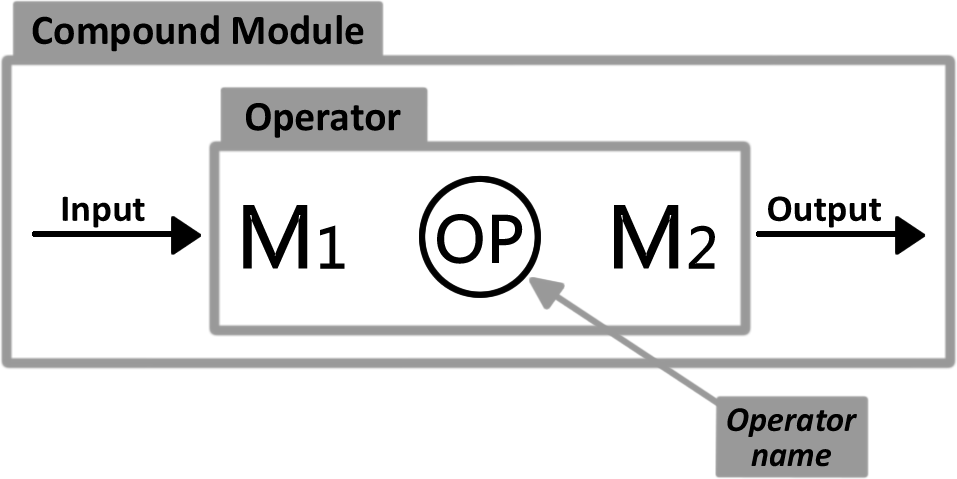
\includegraphics[width=0.7\linewidth]{cm} %[width=0.2\textwidth]{muta1}
	\caption[]{Un \cm}
	\label{fig:cm}
\end{figure}%fr

Dans le  cas particulier  où un  des \cms{}  impliqués est  un \opch{}, chaque opérateur gère l'information {\it NULL} à sa manière.

Afin   de  grouper   des   modules,  nous   utiliserons  la   notation $\left|.\right|$ comme un groupe générique qui pourra être indifféremment interprété comme $[.]$ ou comme $\lbk . \rbk_p$.

Ensuite, les opérateurs fournis par \posl{} sont présentés. 

\underline{\bf Sequential Execution Operator}: \new{L'opération $\left|\mathcal{M}_1\poslop{\mapsto}\mathcal{M}_2\right|$ définit le \cm{} $\mathcal{M}_{seq}$ comme le résultat de l'exécution de $\mathcal{M}_1$ suivi de $\mathcal{M}_2$. C'est un exemple d'opérateur ne  supportant pas une exécution parallèle de ses \cms impliqués, puisque l'entrée du second \cm{} est la sortie du premier.}

\underline{\bf Conditional Execution Operator}: \new{L'opération $\left|\mathcal{M}_1\circled{?}_{<cond>}\mathcal{M}_2\right|$ définit le \cm{} $\mathcal{M}_{cond}$ le résultat de l'exécution en séquentiel de $\mathcal{M}_1$ si $<cond>$ es {\bf vrai} or $\mathcal{M}_2$, autrement.}

\underline{\bf Cyclic Execution Operator}: \new{L'opération $\left|\circlearrowleft_{<cond>}\mathcal{M}\right|$ définit le \cm{} $\mathcal{M}_{cyc}$ en répétant séquentiellement l'exécution de $\mathcal{M}$ tant que $<cond>$ est {\bf vrai}.}

\underline{\bf Random Choice Operator}: \new{L'operation $\left|M_1\circled{$\rho$}\mathcal{M}_2\right|$ définit le \cm{} $\mathcal{M}_{rho}$ qui exécute $\mathcal{M}_1$ en suivant une probabilité $\rho$, ou en exécutant $\mathcal{M}_2$ en suivant une probabilité $(1-\rho)$.}

\underline{\bf Not {\it NULL}}: \new{L'operation $\left|\mathcal{M}_1\circled{$\vee$}\mathcal{M}_2\right|$ définit le \cm{} $\mathcal{M}_{non}$ qui exécute $\mathcal{M}_1$ et retourne une sortie si elle n'est pas {\it NULL}, ou exécute $\mathcal{M}_2$ et retourne une sortie autrement.}

\underline{\bf Minimum Operator}: \new{Soient $o_1$ et $o_2$ les sorties de $\mathcal{M}_1$ et $\mathcal{M}_2$, respectivement. Nous assumons qu'il existe un ordre total dans $I_1 \cup I_2$ où l'objet \emph{NULL} est la plus grand valeur. Alors, l'opération $\left|\mathcal{M}_1\circled{m}\mathcal{M}_2\right|$ définit le \cm{} $\mathcal{M}_{min}$ qui exécute $\mathcal{M}_1$ et $\mathcal{M}_2$, et retourne $\min\left\{o_1,o_2\right\}$.}

\underline{\bf Maximum Operator}: \new{Soient $o_1$ et $o_2$ les sorties de $\mathcal{M}_1$ et $\mathcal{M}_2$, respectivement. Nous assumons qu'il existe un ordre total dans $I_1 \cup I_2$ où l'objet \emph{NULL} est la plus petite valeur. Alors, l'opération $\left|\mathcal{M}_1\circled{M}\mathcal{M}_2\right|$ définit le \cm{} $\mathcal{M}_{max}$ qui exécute $\mathcal{M}_1$ et $\mathcal{M}_2$, et retourne $\max\left\{o_1,o_2\right\}$.}

\underline{\bf Race Operator}: \new{L'opération $\left|\mathcal{M}_1\circled{$\shortdownarrow$}\mathcal{M}_2\right|$ définit le \cm{} $\mathcal{M}_{race}$ qui exécute les deux \ms{} $\mathcal{M}_1$ et $\mathcal{M}_2$, et retourne la sortie du \m{} qui termine en premier}

Les opérateurs $\circled{$\rho$}$, $\circled{$\vee$}$ et $\circled{m}$ sont très  utiles en  terme de  partage d'informations entre   solveurs, mais également en terme de partage de comportements. Si un  des opérandes est un \opch{} alors l'opérateur peut recevoir le \om{} d'un autre solveur, donnant la possibilité d'instancier ce module dans le solveur le réceptionnant. L'opérateur va soit instancier le module s'il  n'est pas {\it NULL} et l'exécuter, soit exécuter le module donné par le second opérande.

Maintenant, nous présentons les opérateurs nous permettant d'envoyer de l'information vers d'autres solveurs. Deux types d'envois sont possibles :
\begin{inparaenum}[i)]
	\item on exécute un \m{} et on envoie sa sortie,
	\item ou on envoie le \m{} lui-même.
\end{inparaenum}

\underline{\bf Sending Data Operator}: \new{L'opération $\left|\senddataop{\mathcal{M}}\right|$ définit le \cm{} $\mathcal{M}_{sendD}$ qui exécute le \m{} $\mathcal{M}$ puis envoie la sortie vers un \opch.}

\underline{\bf Sending Module Operator}: \new{L'opération $\left|\sendmoduleop{\mathcal{M}}\right|$ définit le \cm{} $\mathcal{M}_{sendM}$ qui exécute le \m{} $\mathcal{M}$, puis envoie le \m{} lui même  vers un \opch.}

Avec  les opérateurs  présentés jusqu'ici, nous sommes  en mesure  de concevoir les \ass{} (ou algorithme) de résolution d'un problème de contraintes. Une fois un tel \as{} définie, on peut changer les composants (\oms{} et \opchs) auxquels elle fait appel, permettant ainsi d'implémenter différents solveurs à partir du même \as{} mais composés de différents \ms, du moment que ces derniers respectent la signature attendue, à savoir le types des entrées et sorties.

\new{Un \as{} est déclaré comme suit: après déclarer les noms de l'\mbox{\tet{\bf \as}} ({\it name}), la première ligne définit la liste des \oms{} abstraites ($\mathcal{L}^m$), la seconde ligne, la liste des \opchs{} abstraites ($\mathbf{M}$), puis l'algorithme du solver est définit comment le corps su solver (the root \cm{} $\mathbf{M}$), entre \mbox{\tet{\bf begin}} et \mbox{\tet{\bf end}}.}

\new{Un \as{} peut être déclaré par l'expression régulière suivante:}

\begin{center}
\tet{\bf abstract solver} {\it name} \tet{\bf computation}: $\mathcal{L}^m$ (\tet{\bf communication}: $\mathcal{L}^c$)? \tet{\bf begin} $\mathbf{M}$ \tet{\bf end}
\end{center}

Par exemple, l'algorithme~\ref{algo:as_example} montre l'\as{} correspondant a la figure~\ref{subfig:as}.

\begin{algorithm}[h]
\dontprintsemicolon
\SetNoline
\SetKwProg{myproc}{}{}{}
\myproc{\tet{\bf abstract solver} as\_01\;
\tet{\bf computation} : $I, V, S, A$ \; 
\tet{\bf connection}: $C.M.$}{
	\Begin{
		$I \poslop{\mapsto}$\\
		\While{$\left(\textbf{\Iter < } K_1\right)$}{
			$\left[V\poslop{\mapsto}S\poslop{\mapsto}\left[C.M.\poslop{m} \senddataop{A}\right]\right]$%
		}
	}
}
\caption{Pseudo-code \posl{} pour l'\as{} de la figure~\ref{subfig:as}}\label{algo:as_example}
\end{algorithm}

\subsection{Créer les solveurs}

\new{Maintenant on peut créer les solveurs en instanciant les \ms. Il est possible de faire ceci en spécifiant que un \mbox{\tet{\bf solver}} donné doit implémenter (en utilisant le mot clé \mbox{\tet{\bf implements}}) un \as{} donné, suivi par la liste de \omprefix{} puis \opchs{}. Ces \ms{} doivent correspondre avec les signatures exigé par l'\as.}

\begin{algorithm}[h]
\dontprintsemicolon
\SetNoline
\SetKwProg{myproc}{}{}{}
\tet{\bf solver} solver\_01 \tet{\bf implements} as\_01\;
\tet{\bf computation} : $I_{rand}, V_{1ch}, S_{best}, A_{AI}$ \; 
\tet{\bf connection}: $CM_{last}$\;
\caption{Une instanciation de l'\as{} présenté dans l'algorithme~\ref{algo:as_example}}\label{algo:solver_def}
\end{algorithm}

\subsection{Connecter les solveurs : créer le \soset}

\new{La dernière étape est connecter les solveurs entre eux. \posl{} fournit des outils pour créer des stratégies de communication très facilement. L'ensemble des solveurs connectés qui seront exécutés en parallèle pour résoudre un CSP s'appelle \INTROsoset{}.}

Les communications sont établies en respectant les règles suivantes :
\begin{enumerate}
\item  À chaque  fois qu'un  solveur  envoie une  information via  les opérateurs  $\llparenthesis .\rrparenthesis^{d}$  ou $\llparenthesis   .\rrparenthesis^{m}$, il créé une {\it prise mâle de communication} 
\item À  chaque fois qu'un  solveur contient  un \opch{}, il  créé une {\it prise femelle de communication} 
\item Les solveurs peuvent être connectés entre eux en reliant {\it prises mâles} et {\it femelles}.
\end{enumerate}

Avec l'opérateur~$(\cdot)$, nous  pouvons  avoir  accès aux  \oms{} envoyant une information et aux noms des \opchs d'un solveur. Par exemple : $Solver_1\cdot\mathcal{M}_1$ fournit  un accès à le \om{} $\mathcal{M}_1$ du $Solver_1$ si et seulement s'il est utilisé par l'opérateur  $\llparenthesis .\rrparenthesis^{d}$  (ou $\llparenthesis.\rrparenthesis^{m}$), et $Solver_2\cdot\mathcal{C}h_2$ fournit un accès au \opch{} $\mathcal{C}h_2$ de $Solver_2$.

Maintenant, nous définissons les opérateurs de communication que \posl{} fournit.

\begin{definition}\label{op_conn:1to1}
{\bf Connection One-to-One Operator} Soient
\begin{enumerate}
\item $\mathcal{J} = \left[\mathcal{S}_0\cdot \mathcal{M}_0, \mathcal{S}_1\cdot \mathcal{M}_1,\dots, \mathcal{S}_{N-1}\cdot \mathcal{M}_{N-1}\right]$ une liste de  {\it prises mâles}, et
\item $\mathcal{O} = \left[\mathcal{Z}_0\cdot \mathcal{CM}_0, \mathcal{Z}_1\cdot \mathcal{CM}_1,\dots, \mathcal{Z}_{N-1}\cdot \mathcal{CM}_{N-1}\right]$ une liste de {\it prises femelles}
\end{enumerate} Alors, l'opération
\[
\mathcal{J} \poslop{\rightarrow} \mathcal{O}
\]
\new{connecte chaque {\it prise mâles} $\mathcal{S}_i\cdot \mathcal{M}_i \in \mathcal{J}$ avec la correspondante {\it prise femelle} $\mathcal{Z}_i\cdot \mathcal{CM}_i \in \mathcal{O}$, $\forall\textbf{ }0 \leq i \leq N-1$ (voir figure~\ref{subfig:comm_simple}).}
\end{definition}

\begin{definition}\label{op_conn:1ton}
{\bf Connection One-to-N Operator} Soient 
\begin{enumerate} 
\item $\mathcal{J} = \left[\mathcal{S}_0\cdot \mathcal{M}_0, \mathcal{S}_1\cdot \mathcal{M}_1,\dots, \mathcal{S}_{N-1}\cdot \mathcal{M}_{N-1}\right]$ une liste de  {\it prises mâles}, et
\item $\mathcal{O} = \left[\mathcal{Z}_0\cdot \mathcal{CM}_0, \mathcal{Z}_1\cdot \mathcal{CM}_1,\dots, \mathcal{Z}_{M-1}\cdot \mathcal{CM}_{M-1}\right]$ une liste de {\it prises femelles}
\end{enumerate} Alors, l'opération
\[
\mathcal{J} \poslop{\rightsquigarrow} \mathcal{O}
\]
\new{connecte chaque {\it prise mâles} $\mathcal{S}_i\cdot \mathcal{M}_i \in \mathcal{J}$ avec chaque {\it prise femelle} $\mathcal{Z}_j\cdot \mathcal{CM}_j \in \mathcal{O}$, $\forall\textbf{ }0 \leq i \leq N-1$ et $0 \leq j \leq M-1$ (see Figure~\ref{subfig:comm_diff}).}
\end{definition}


\posl{} permet aussi de déclarer des solveurs non communicatifs pour les exécuter en parallèle, en déclarant seulement la liste des noms:
\[
\left[\mathcal{S}_0, \mathcal{S}_1, \dots, \mathcal{S}_{N-1}\right]
\]

\begin{figure}[h]
\centering
\subfloat[][Communication 1 à 1]{
	\label{subfig:comm_simple}
	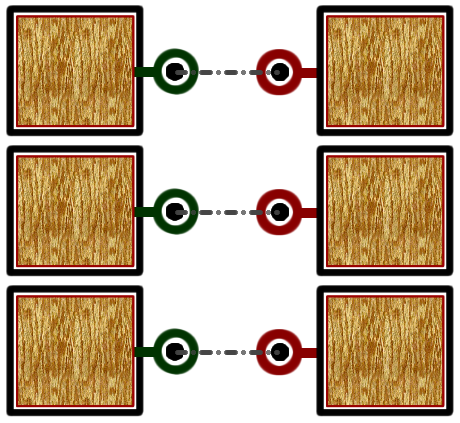
\includegraphics[width=0.4\columnwidth]{comm_11.png}
}
\hspace{0.05\textwidth}%
\subfloat[][Communication 1 à N]{%
	\label{subfig:comm_diff}
	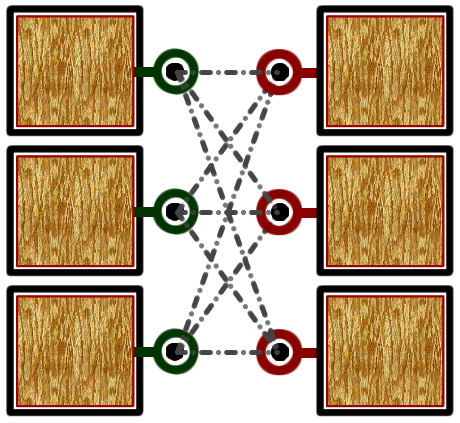
\includegraphics[width=0.4\columnwidth]{comm_1n.png}
}
\caption[]{Représentation graphique des opérateurs de communication}
\label{fig:comm}
\end{figure}



























































\section{Les résultats}

Le but principal de cette section est de sélectionner quelques instances de problèmes de référence, pour analyser et illustrer la versatilité de \posl{} pour étudier des stratégies de solution basées sur la recherche locale méta-heuristique avec communication. Grâce à \posl{} nous pouvons analyser des résultats et formuler des conclusions sur le comportement de la stratégie de recherche, mais aussi sur la structure de l'espace de recherche du problème. Dans cette section, nous expliquons la structure des  solveurs de \posl{} que nous avons générés pour les expériences, et les résultats.

Nous avons choisi l'une des méthodes de solutions les plus classique pour des problèmes combinatoires: l'algorithme méta-heuristique de recherche locale. Ces algorithmes ont une structure commune: ils commencent par l'initialisation des structures de données. Ensuite, une configuration initiale $s$ est générée. Après cela, une nouvelle configuration $s'$ est sélectionnée dans le voisinage $V \left(s \right) $. Si $s'$ est une solution pour le problème $P$, alors le processus s'arrête, et $s'$ est renvoyée. Dans le cas contraire, les structures de données sont mises à jour, et $s'$ est acceptée, ou non, pour l'itération suivante, en fonction de certains critères (par exemple, en pénalisant les caractéristiques des optimums locaux).

Les expériences ont été effectuées sur un processeur Intel \R{} Xeon \TM{} E5-2680 v2, 10 $\times$ 4 c\oe urs, 2.80GHz. Les résultats montrés dans cette section sont les moyennes de 30 runs pour chaque configuration. Dans les tableaux de résultats, les colonnes marquées {\bf T} correspondent au temps de l'exécution en secondes et les colonnes marquées {\bf It.} correspondent au nombre d'itérations. Toutes les expériences de cette section sont basées sur différentes stratégies en parallèle, avec 40 c\oe urs.

\subsection{Social Golfers Problem}

Le problème de \sg{} (\SGP) consiste à planifier $n = g \times p$ golfeurs en $g$ groupes de $p$ joueurs chaque semaine pendant $w$ semaines, de telle manière que deux joueurs jouent dans le même groupe au plus une fois. Une instance de ce problème peut être représentée par le triplet $g-p-w$. Ce problème, et d'autres problèmes étroitement liés, trouvent de nombreuses applications pratiques telles que le codage, le cryptage et les problèmes couvrants. Sa structure nous a semblé intéressante car elle est similaire à d'autres problèmes, comme {\it Kirkman's Schoolgirl} et {\it Steiner Triple System}, donc nous pouvons construire des modules efficaces pour résoudre un grand éventail de problèmes.

Nous avons utilisé uns stratégie de communication cyclique pour résoudre ce problème, en échangeant la configuration courante entre deux solveurs avec des caractéristiques différentes. Les résultats montrent que cette stratégie marche très bien pour ce problème.

\begin{algorithm}
\dontprintsemicolon
\scriptsize
\SetNoline
\SetKwProg{myproc}{\tet{\bf abstract solver}}{\tet{\bf begin}}{\tet{\bf end}}
\myproc{as\_eager \tcp*{{\sc Itr} $\rightarrow$ nombre d'itérations}
	\tet{\bf computation} : $I, V, S_1, S_2, A$\;\tcp*{{\sc Sci} $\rightarrow$ nombre d'itérations avec le même coût}}{%
	$I \poslop{\mapsto}$\\
	\While{$\left(\textbf{\Iter} < K_1\right)$}{
		$V \poslop{\mapsto} \left[S_1 \poslopcond{\Sci \% K_2} S_2\right] \poslop{\mapsto} A$		
	}
}
\tet{\bf solver} \solverposl{eager} \tet{\bf implements} as\_eager\;
\algoindent \tet{\bf computation} : $I_{BP}, V_{BAS}, S_{first}, S_{rand}, A_{AI}$ \;
\caption{Solveur pour \SGP}\label{as:golfers_eager}
\end{algorithm}

L'algorithme~\ref{as:golfers_eager} montre l'\as{} utilisé pour résoudre me manière séquentielle le \SGP{}. L'utilisation de deux \ms{} de sélection ($S_1$ et $S_2$) est un simple chamanisme pour éviter les minimums locaux: il tente d'améliorer le coût un certain nombre de fois, en exécutant le \om{} $S_1$. S'il n'y arrive pas, il exécute le \om{} $S_2$. L'\as{} a été instancié par les \oms{} suivantes:

\begin{enumerate}
\item $S_{BP}$ génère une configuration aléatoire $s$, en respectant la structure du problème, c'est-à-dire que la configuration est un ensemble de $w$ permutations du vecteur $[1..n]$.
\item $V_{BAS}$ définit le voisinage $V \left(s\right)$ permutant le joueur qui a contribué le plus au coût, avec d'autres joueurs dans la même semaine.
\item $S_{rirst}$ sélectionne la première configuration $s'\in V\left (s\right)$ qui améliore le coût actuel, et retourne $(s, s')$
\item $S_{rand}$ sélectionne une configuration aléatoire $s'\in V\left(s\right)$, et retourne $(s, s')$
\item $A_{AI}$ retourne toujours la configuration sélectionnée ($s'$).
\end{enumerate}

Pour \SGP{}, nous avons utilisé une stratégie de communication, où un solveur "compagnon", incapable de trouver une solution au final, mais capable de trouver des configurations avec an coût considérablement plus petit que ceci trouvé par le solveur \textit{standard} dans le même instant de temps, au début de la recherche. L'idée c'est d'échanger leurs configurations cycliquement, jusqu'à trouver une solution. Les algorithmes~\ref{as:golfers_full} et \ref{as:golfers_partial} montrent les solveurs utilisés pour cette stratégie, ou $V_{BP}(p)$ est le \om{} de voisinage pour le solveur "compagnon", qui cherche des configurations seulement changeant des joueurs parmi $p$ semaines. Le \opch{} instancié $CM_{last}$, prend en compte la dernière configuration reçue quand il est au moment de l'exécution.

\begin{algorithm}
\dontprintsemicolon
\scriptsize
\SetNoline
\SetKwProg{myproc}{\tet{\bf abstract solver}}{\tet{\bf begin}}{\tet{\bf end}}
\myproc{as\_standard \; %\hspace{3pt}
	\tet{\bf computation} : $I, V, S_1, S_2, A$ \; %\hspace{3pt}
	\tet{\bf communication} : $C.M.$\;}{%
	$I \poslop{\mapsto}$\\
	\While{$\left(\textbf{\Iter} < K_1\right)$}{
		$V \poslop{\mapsto} \left[S_1 \poslopcond{\Sci \% K_2} S_2\right] \poslop{\mapsto} \left[C.M. \poslop{m} \llparenthesis A \rrparenthesis^d\right]$		
	}
}
\tet{\bf solver} \solverposl{standard} \tet{\bf implements} as\_standard\;
\algoindent \tet{\bf computation} : $I_{BP}, V_{BAS}, S_{first}, S_{rand}, A_{AI}$ \;
\algoindent \tet{\bf communication} : $CM_{last}$ \;
\caption{Solveur standard pour \SGP}\label{as:golfers_full}
\end{algorithm}

\begin{algorithm}
\dontprintsemicolon
\scriptsize
\SetNoline
\SetKwProg{myproc}{\tet{\bf abstract solver}}{\tet{\bf begin}}{\tet{\bf end}}
\myproc{as\_compagnon \; %\hspace{1pt}
	\tet{\bf computation} : $I, V, S_1, S_2, A$ \;
	\tet{\bf communication} : $C.M.$\;}{
	$I \poslop{\mapsto}$\\
	\While{$\left(\textbf{\Iter} < K_1\right)$}{
		$V \poslop{\mapsto} \left[S_1 \poslopcond{\Sci \% K_2} S_2\right] \poslop{\mapsto} \left[C.M. \poslop{\vee} \llparenthesis A \rrparenthesis^d\right]$		
	}
}
\tet{\bf solver} \solverposl{compagnonandard} \tet{\bf implements} as\_compagnon\;
\algoindent \tet{\bf computation} : $I_{BP}, V_{BP}(p), S_{first}, S_{rand}, A_{AI}$ \;
\algoindent \tet{\bf communication} : $CM_{last}$ \;
\caption{Solveur compagnon pour \SGP}\label{as:golfers_partial}
\end{algorithm}

Nous avons dessiné aussi des différentes stratégies de communication, en combinant des solveurs connectés et non-connectés, et en appliquant des différents opérateurs de communication : \oneTone{} et \oneTn.

\begin{table}[t]
\centering
\renewcommand{\arraystretch}{1}
\resizebox{\columnwidth}{!}{%
\begin{tabular}{p{1.4cm}|R{1cm}R{1cm}|R{1cm}R{1cm}|R{1.3cm}R{1.3cm}}
\hline
{\bf Instance} & \multicolumn{2}{c|}{\textbf{Séquentielle}} & \multicolumn{2}{c|}{\textbf{Parallèle}} & \multicolumn{2}{c}{\textbf{Coopérative}}\\
\cline{2-7}
 & T & It. & T & It. & T & It.\\
\hline
%\hline
5--3--7 & 1.25 & 2,903 & 0.23 & 144 & \good{0.10} & 98\\
8--4--7 & 0.60 & 338 & 0.28 & 93 & \good{0.14} & 54\\
9--4--8 & 1.04 & 346 & 0.59 & 139 & \good{0.36} & 146\\
\hline
\end{tabular}
}
\caption{Résultats pour \SGP}
\label{tab:golfers_seqpar}
\end{table}

Comme nous nous attendions, le tableau~\ref{tab:golfers_seqpar} confirme le succès de l'approche parallèle sur le séquentielle. Plus intéressante, les expériences confirment que la stratégie de communication proposée pour cet benchmark est la correcte: en comparant par rapport aux runs en parallèle sans communication, il améliore les runtimes par un facteur de 1.98 (facteur moyen parmi les trois instances). Les résultats coopératifs de ce tableau on été obtenus en utilisant l'opérateur de communication \oneTone{} avec 100\% de solveurs communicatifs. 


\subsection{Costas Array Problem}

Le problème \carr{} (\CARRP) consiste à trouver une matrice {\it Costas}, qui est une grille de $n \times n$ contenant $n$ marques avec exactement une marque par ligne et par colonne et les $n(n-1)/2 $ vecteurs reliant chaque couple de marques de cette grille doivent tous être différents. Ceci est un problème très complexe trouvant une application utile dans certains domaines comme le sonar et l'ingénierie de radar, et présente de nombreux problèmes mathématiques ouverts. Ce problème a aussi une caractéristique intéressante: même si son espace de recherche grandit factoriellement, à partir de l'ordre 17 le nombre de solutions diminue drastiquement.

Pour ce problème nous avons testé une stratégie de communication simple, où l'information a communiquer est la configuration courante. Pour construire les solveurs, nous avons réutilisé les \oms{} de sélection ($S_{first}$) et de d'acceptation ($S_{AI}$) et le \opch{} utilisés dans la résolution de \SGP{}. Les autres \oms{} sont les suivantes :

\begin{enumerate}
	\item $I_{perm}$: génère une configuration aléatoire $s$, comme une permutation du vecteur $[1..n]$. 
	\item $V_{AS}$: définit le voisinage $V \left(s\right)$ permutant la variable qui a contribué le plus au coût, avec d'autres.
\end{enumerate}

Pour résoudre \CARRP{} nous avons eu besoin d'utiliser un \om{} de \textit{reset} ($T_{AS}$) comme machinisme d'exploration. L'algorithme~\ref{as:costas} montre le solveur utilisé pour résoudre ce problème séquentiellement. Les résultats des runs en séquentiel et en parallèle sans communication sont montrés dans le tableau~\ref{tab:costas19}. Ils montrent le succès de l'approche en parallèle est montré encore une fois. Afin d'améliorer ces résultats, nous avons appliqué uns stratégies   simple de communication : communiquer la configuration courante au moment d'exécuter le critère d'acceptation. Les algorithmes~\ref{as:costas_sender} et~\ref{as:costas_receiver} montrent les solveurs envoyeur et récepteur.

\begin{algorithm}
\dontprintsemicolon
\scriptsize
\SetNoline
\SetKwProg{myproc}{\tet{\bf abstract solver}}{\tet{\bf begin}}{\tet{\bf end}}
\myproc{as\_hard \;
	\tet{\bf computation} : $I, T, V, S, A$\;}{
	$I \poslop{\mapsto}$\\
	\While{$\left(\textbf{\Iter} < K_1\right)$}{
		$T \poslop{\mapsto}$
		\whileinline{$\left(\textbf{\Iter \% } K_2\right)$}{$\left[V \poslop{\mapsto} S \poslop{\mapsto} A\right]$}
	}
}
\tet{\bf solver} \solverposl{1} \tet{\bf implements} as\_hard\;
\algoindent\tet{\bf computation} : $I_{perm}, T_{AS}, V_{AS}, S_{first}, A_{AI}$ \;
\caption{Solveur pour \CARRP}\label{as:costas}
\end{algorithm}

\begin{table}[t]
\captionsetup{belowskip=6pt,aboveskip=6pt}
\centering
\renewcommand{\arraystretch}{1}
\resizebox{\columnwidth}{!}{%
\begin{tabular}{p{3.2cm}|R{1.2cm}R{1.5cm}R{1.5cm}}
	\hline
	{\bf STRATÉGIE} & T & It. & \% success\\
	\hline
	%\hline
	Séquentielle  & 132.73 & 2,332,088 & 40.00\\
	Parallèle & 25.51 & 231,262 & 100.00\\
	Coopérative & \good{10.83} & \good{79,551} & 100.00\\
	\hline
\end{tabular}
}
\caption{Résultats pour \CARRP{} 19}
\label{tab:costas19}
\end{table}

\begin{algorithm}
\dontprintsemicolon
\scriptsize
\SetNoline
\SetKwProg{myproc}{\tet{\bf abstract solver}}{\tet{\bf begin}}{\tet{\bf end}}
\myproc{as\_hard\_sen \; 
	\tet{\bf computation} : $I, T, V, S, A$\;}{
	$I \poslop{\mapsto}$\\
	\While{$\left(\textbf{\Iter} < K_1\right)$}{
		$T \poslop{\mapsto}$
		\whileinline{$\left(\textbf{\Iter \% } K_2\right)$}{$\left[V \poslop{\mapsto} S \poslop{\mapsto} \llparenthesis A \rrparenthesis^d\right]$}
	}
}
\tet{\bf solver} \solverposl{sender} \tet{\bf implements} as\_hard\_sen\;
\algoindent\tet{\bf computation} : $I_{perm}, T_{AS}, V_{AS}, S_{first}, A_{AI}$ \;
\caption{Solveur envoyeur pour \CARRP}\label{as:costas_sender}
\end{algorithm}

\begin{algorithm}
\dontprintsemicolon
\scriptsize
\SetInd{2pt}{2pt}
\SetNoline
\SetKwProg{myproc}{\tet{\bf abstract solver}}{\tet{\bf begin}}{\tet{\bf end}}
\myproc{as\_hard\_rec \; 
	\tet{\bf computation} : $I, T, V, S, A$ \; 
	\tet{\bf communication} : $C.M.$\;}{ 
	$I \poslop{\mapsto}$\\
	\While{$\left(\textbf{\Iter} < K_1\right)$}{
		$T \poslop{\mapsto}$
		\whileinline{$\left(\textbf{\Iter \% } K_2\right)$}{$\left[V \poslop{\mapsto} S \poslop{\mapsto} \left[A\poslop{m}C.M.\right]\right]$}
	}
}
\tet{\bf solver} \solverposl{receiver} \tet{\bf implements} as\_hard\_rec\;
\algoindent\tet{\bf computation} : $I_{perm}, T_{AS}, V_{AS}, S_{first}, A_{AI}$ \; 
\algoindent\tet{\bf communication}: $CM_{last}$\;
\caption{Solveur récepteur pour \CARRP}\label{as:costas-receiver}
\end{algorithm}

Un des buts principaux de cette étude a été d'explorer des différentes stratégies de communication. Nous avons ensuite mis en place et testé différentes variantes de la stratégie exposée ci-dessus en combinant deux opérateurs de communication (\oneTone{} et \oneTn) et des pourcentages différents de solveurs communicantes. Comme prévu, la meilleure stratégie était basée sur 100\% de communication avec l'opérateur \oneTn{}, parce que cette stratégie permet de communiquer un lieu prometteur à l'intérieur de l'espace de recherche à un maximum de solveurs, en refor\c{c}ant  l'intensification.

\subsection{Golomb Ruler Problem}

Le \grp{} (\GRP) consiste à trouver un vecteur ordonné de $n$ entiers non négatifs différents, appelés \textit{marques}, $m_1<\dots<m_n$, tel que toutes les différences $m_i- m_j$, $(i>j)$ sont toutes différentes. Une instance de ce problème est défini par le paire $(o,l)$ où $o$ est l'ordre du problème, (le nombre de \textit{marques}) et  $l$ est la longueur de la règle (la dernière {\it marque}). Nous supposons que la première \textit{marque} est toujours 0. Lorsque nous appliquons \posl{} pour résoudre une instance de problème séquentiellement, nous pouvons remarquer qu'il effectue de nombreux {\it restars} avant de trouver une solution. Pour cette raison, nous avons choisi ce problème pour étudier une stratégie de communication intéressante: communiquer la configuration actuelle afin d'éviter son voisinage, c'est à dire, une configuration {\it tabu}.

Nous réutilisons les \ms{} de sélection et d'acceptation des études antérieures ($S_{first}$ et$A_{AI}$) pour concevoir les \ass. Les nouvelles \ms{} sont:
\begin{enumerate}
\item $I_{sort}$: renvoie une configuration aléatoire $s$ en tant que vecteur d'entiers trié. La configuration est générée \textit{loin} de l'ensemble des configurations {\it tabu} arrivés via communication entre solveurs.
\item $V_{sort}$: donné une configuration, retourne le voisinage en changeant une valeur tout en gardant l'ordre, à savoir, le remplacement de la valeur $s_i$ par toutes les valeurs possibles $s'_i \in D_i$ en satisfaisant $s_{i-1}< s'_i < s_{i+1}$.
\end{enumerate}

Nous avons également ajouté un module de reset $T$: il reçoit et renvoie une configuration. Le \om{} utilisé pour l'instancier ($T_{tabu}$) insère la configuration reçue dans une liste \textit{tabu} à l'intérieur du solveur et retourne la configuration d'entrée \modified{tal cual}. L'algorithme~\ref{as:golomb_sender} présente le solveur utilisé pour envoyer des informations (solveur envoyeur).

\begin{algorithm}
\dontprintsemicolon
\scriptsize
\SetNoline
\SetKwProg{myproc}{\tet{\bf abstract solver}}{\tet{\bf begin}}{\tet{\bf end}}
\myproc{as\_golomb\_sender\;
	\tet{\bf computation} : $I, V, S, A, T$\;}{
	\While{$\left(\textbf{\Iter} < K_1\right)$}{
		$I \poslop{\mapsto}$ 
		\whileinline{$\left(\textbf{\Iter \% } K_2\right)$}{$\left[V \poslop{\mapsto} S \poslop{\mapsto} A\right]$} $\poslop{\mapsto} \llparenthesis T \rrparenthesis^d$
	}
}
\tet{\bf solver} \solverposl{sender} \tet{\bf implements} as\_golomb\_sender\;
\algoindent\tet{\bf computation} : $I_{sort}, V_{sort}, S_{first}, A_{AI}, , T_{tabu}$ \; 
\caption{Solveur envoyeur pour  \GRP}\label{as:golomb_sender}
\end{algorithm}

Le module $T_{tabu}$ est exécuté lorsque le solveur est incapable de trouver une meilleure configuration autour de l'actuelle: elle est supposée être un minimum local, et elle est envoyée au solveur récepteur. L'algorithme~\ref{as:golomb_receiver} présente solveur utilisé pour recevoir l'information. Le \opch{} $CM_{set}$ reçoit plusieurs configurations qui sont reçus par le \om{} $I_{sort}$ comme entrées.
 
\begin{algorithm}
\dontprintsemicolon
\scriptsize
\SetNoline
\SetKwProg{myproc}{\tet{\bf abstract solver}}{\tet{\bf begin}}{\tet{\bf end}}
\myproc{as\_golomb\_receiver\;
	\tet{\bf computation} : $I, V, S, A, T$\;
	\tet{\bf connection} : $C.M.$\;}{
	\While{$\left(\textbf{\Iter} < K_1\right)$}{
		$\left[C.M. \poslop{\mapsto} I \right] \poslop{\mapsto}$ \\
		\whileinline{$\left(\textbf{\Iter \% } K_2\right)$}{$\left[V \poslop{\mapsto} S \poslop{\mapsto} A\right]$} $\poslop{\mapsto} T$
	}
}
\tet{\bf solver} \solverposl{receiver} \tet{\bf implements} as\_golomb\_receiver\;
\algoindent\tet{\bf computation} : $I_{sort}, V_{sort}, S_{first}, A_{AI}, , T_{tabu}$ \; 
\algoindent\tet{\bf communication}: $CM_{set}$\;
\caption{Solveur récepteur pour \GRP}\label{as:golomb_receiver}
\end{algorithm}

Le bénéfice de l'approche en  parallèle avec \posl{} est aussi prouvé pour le \GRP{} (voir les tableaux~\ref{tab:golomb_seq} et~\ref{tab:golomb_seq}). Dans ces tableaux, la colonne \textbf{R} représente le nombre de redémarrages exécutées. Cette expérience a été réalisée en utilisant des solveurs similaires à ceux présentés précédemment, mais sans \opchs.

\begin{table}
\captionsetup{belowskip=6pt,aboveskip=6pt}
\centering 
\renewcommand{\arraystretch}{1}
%\resizebox{\columnwidth}{!}{%
\begin{tabular}{p{1.4cm}|R{1.1cm}R{1.3cm}R{0.6cm}R{1.5cm}}
\hline
{\bf Instance} & T & It. & R & \% success \\
\hline
%\hline
8--34 & 0.66 & 10,745 & 53 & 100.00 \\
10--55 & 67.89 & 446,913 & 297 & 88.00 \\
11--72 & 117.49 & 382,617 & 127 & 30.00 \\
\hline
\end{tabular}
%}
\caption{Résultats séquentielles pour \GRP{}}
\label{tab:golomb_seq}
\end{table}

\begin{table}
\captionsetup{belowskip=6pt,aboveskip=6pt}
\centering 
\renewcommand{\arraystretch}{1}
%\resizebox{\columnwidth}{!}{%
\begin{tabular}{p{1.4cm}|R{0.9cm}R{1.3cm}R{0.6cm}}
\hline 	
{\bf Instance} & T & It. & R \\
\hline
%\hline
8--34 & 0.43 & 349 & 1\\
10--55 & 4.92 & 20,504 & 13\\
11--72 & 85.02 & 155,251 & 51\\
\hline
\end{tabular}
%}
\caption{Résultats en parallèle non coopératifs pour \GRP{}}
\label{tab:golomb_par}
\end{table}

Pour \GRP, la stratégie de communication que nous adoptions a été différente. L'idée de cette stratégie est de profiter des nombreux redémarrages indiqués dans les tableaux~\ref{tab:golomb_seq} et~\ref{tab:golomb_par}. Chaque fois qu'un solveur redémarre, la configuration actuelle est communiquée pour alerter les solveurs et éviter son voisinage. De cette façon, chaque fois qu'un solveur redémarre, il génère une nouvelle configuration assez loin de ces "zones pénalisées".

Sur la base de l'opérateur de connexion utilisé dans la stratégie de communication, ce solveur peut recevoir une ou plusieurs configurations. Ces configurations sont l'entrée du \m{} de génération ($I_{sort}$). Ce module insère toutes les configurations reçues dans une liste {\it tabu}, puis il génère une nouvelle première configuration loin de toutes les configurations dans la liste {\it tabu}. 

Comme nous pouvons voir dans les tableaux~\ref{tab:golomb_comm_notab} et~\ref{tab:golomb_comm_tab} l'amélioration en temps d'exécution avec communication est plus visible quand on utilise l'opérateur de communication \oneTn{}, parce-que à chaque nouvelle itération, le solveur récepteur a plus d'information afin de générer une nouvelle configuration loin des "zones pénalisées".

\begin{table}[t]
\captionsetup{belowskip=6pt,aboveskip=6pt}
\centering 
\renewcommand{\arraystretch}{1}
\begin{tabular}{p{1.4cm}|R{0.9cm}R{1.2cm}R{0.8cm}}
	\hline 	
	{\bf Instance} & T & It. & R \\
	\hline
	8--34 & 0.44 & 309 & 1 \\
	10--55 & 3.90 & 15,437 & 10 \\
	11--72 & 85.43 & 156,211 & 52 \\
	\hline
\end{tabular}
\caption{Résultats avec communication sans liste tabu pour \GRP.}
\label{tab:golomb_comm_notab}
\end{table}

\begin{table}[t]
\captionsetup{belowskip=6pt,aboveskip=6pt}
\centering 
\renewcommand{\arraystretch}{1}
\begin{tabular}{p{1.4cm}|R{1cm}R{1.3cm}R{0.8cm}}
	\hline 	
	{\bf Instance} & T & It. & R \\
	\hline
	8--34 & \good{0.43} & 283 & 1\\
	10--55 & \good{3.16} & 12,605 & 8\\
	11--72 & \good{60.35} & 110,311 & 36\\
	\hline
\end{tabular}
\caption{Résultats avec communication avec liste tabu pour \GRP.}
\label{tab:golomb_comm_tab}
\end{table}

\section{Conclusions}

Dans cette thèse, nous avons  présenté \posl{}, un système pour construire des solveurs parallèles coopératifs. Il propose une manière modulable  pour créer   des  solveurs   capables   d'échanger   n'importe  quel   type d'informations, comme par exemple leur comportement même, en partageant
leurs \oms.  Avec \posl{},  de nombreux solveurs  différents pourront être créés et  lancés en parallèle, en utilisant  une unique stratégie générique mais en instanciant différents  \oms{} et \opchs{} pour chaque solveur. 

Il est possible d'implémenter différentes stratégies de communication, puisque  \posl{} fournit une couche pour définir les canaux de communication connectant les solveurs entre eux.

Nous avons présenté aussi des résultats en utilisant \posl{} pour résoudre des instances des problèmes classiques CSP. Il a été possible d'implémenter différentes stratégies communicatives et non communicatives, grâce au langage basé sur des opérateurs fournis, pour combiner différents \oms{}. \posl{} donne la possibilité de relier dynamiquement des solveurs, étant capable de définir des stratégies différentes en terme de pourcentage de solveurs communicatifs. Les résultats montrent la capacité de \posl{} à résoudre ces problèmes, en montrant en même temps que la communication peut jouer un rôle décisif dans le processus de recherche.

\posl{} a déjà une importante bibliothèque de \oms{} et de \opchs{} prête à utiliser, sur la base d'une étude approfondie sur les algorithmes méta-heuristiques classiques pour la résolution de problèmes combinatoires. Dans un avenir proche, nous prévoyons de la faire grandir, afin d'augmenter les capacités de \posl.

En même temps, nous prévoyons d'enrichir le langage en proposant de nouveaux opérateurs. Il est nécessaire, par exemple, d'améliorer le langage de {\it définition du solveur}, pour permettre la construction plus rapide et plus facile des ensembles de nombreux nouveaux solveurs. En plus, nous aimerions élargir le langage des opérateurs de communication, afin de créer des stratégies de communication polyvalentes et plus complexes, utiles pour étudier le comportement des solveurs.

\bibliography{biblio201608}

\end{document}
